\documentclass[12pt,a4paper]{article}
\def\version{6.1}
\def\qe{{\sc Quantum ESPRESSO}}
\def\qeforge{\texttt{qe-forge.org}}
\textwidth = 17cm
\textheight = 24cm
\topmargin =-1 cm
\oddsidemargin = 0 cm


% BEWARE: don't revert from graphicx for epsfig, because latex2html
% doesn't handle epsfig commands !!!
\usepackage{graphicx}
\usepackage{amssymb}

\def\configure{\texttt{configure}}
\def\configurac{\texttt{configure.ac}}
\def\autoconf{\texttt{autoconf}}

\def\pwx{\texttt{pw.x}}
\def\phx{\texttt{ph.x}}
\def\configure{\texttt{configure}}
\def\PWscf{\texttt{PWscf}}
\def\PHonon{\texttt{PHonon}}
\def\make{\texttt{make}}

\begin{document} 
\author{}
\date{}
\title{
  \vskip 1cm
  % title
  \Huge Points inside the Brillouin zone \\
  \Large Notes by Andrea Dal Corso (SISSA - Trieste)
}
\maketitle

\newpage

\section{Brillouin zone}

\qe\ (QE) support for the definition of high symmetry lines inside the Brillouin
zone (BZ) is still rather limited. However QE can calculate the coordinates 
of the vertexes of the BZ and of particular points inside the BZ. These 
notes show the shape and orientation of the BZ used by QE. The principal 
direct and reciprocal lattice vectors, as implemented 
in the routine \texttt{latgen}, are illustrated here together with the labels 
of each point. These labels can be given as input in a band or phonon 
calculation to define paths in the BZ. This feature is available with 
the option \texttt{tpiba\_b} or \texttt{crystal\_b} in a \texttt{'bands'} 
calculation or with the option \texttt{q\_in\_band\_form} in the input of the 
\texttt{matdyn.x} code.
BEWARE: you need to explicitly specify \texttt{ibrav} to use this feature.
Lines in reciprocal space are defined by giving the coordinates of the 
starting and ending points and the number of points of each line.
The coordinates of the starting and ending points can be 
given explicitly with three real numbers or by giving the label of a 
point known to QE.
For example:
\begin{verbatim}
X  10
gG 25
0.5 0.5 0.5 1
\end{verbatim}
indicate a path composed by two lines. The first line starts at point $X$,
ends at point $\Gamma$, and has $10$ {\bf k} points. The second line starts
at $\Gamma$, ends at the point of coordinates \texttt{(0.5,0.5,0.5)} and
has $25$ {\bf k} points. Greek labels are prefixed by the letter
\texttt{g}: \texttt{gG} indicates the $\Gamma$ point, \texttt{gS} the 
$\Sigma$ point etc. Subscripts are written after the label: the point $P_1$ 
is indicated as \texttt{P1}. In the following section you can find the
labels of the points defined in each BZ. 
There are many conventions to label high symmetry
points inside the BZ. The variable \texttt{point\_label\_type} selects the
set of labels used by QE. The default is \texttt{point\_label\_type='SC'} and
the labels have been taken from W. Setyawan and S. Curtarolo, Comp. Mat. Sci.
{\bf 49}, 299 (2010). Other choices can be more convenient in other situations. 
The names reported in the web pages 
\texttt{http://www.cryst.ehu.es/cryst/get\_kvec.html}
are available for some BZ. You can use them by setting
(\texttt{point\_label\_type='BI'}), others can be added in the future.
This option is available only with \texttt{ibrav$\ne$0} and for 
all positive \texttt{ibrav} with the exception of the base centered 
monoclinic (\texttt{ibrav=13}), and triclinic (\texttt{ibrav=14}) lattices. 
In these cases you have to give all the coordinates of the {\bf k}-points.

\subsection{\texttt{ibrav=1}, simple cubic lattice}
The primitive vectors of the direct lattice are:
\begin{eqnarray}
{\bf a}_1 &=& a (1, 0, 0), \nonumber \\
{\bf a}_2 &=& a (0, 1, 0), \nonumber \\
{\bf a}_3 &=& a (0, 0, 1), \nonumber
\nonumber
\end{eqnarray}
while the reciprocal lattice vectors are:
\begin{eqnarray}
{\bf b}_1 &=& {2\pi \over a} (1, 0, 0), \nonumber \\
{\bf b}_2 &=& {2\pi \over a} (0, 1, 0), \nonumber \\
{\bf b}_3 &=& {2\pi \over a} (0, 0, 1). \nonumber
\nonumber
\end{eqnarray}
The Brilloin zone is:
\begin{center}
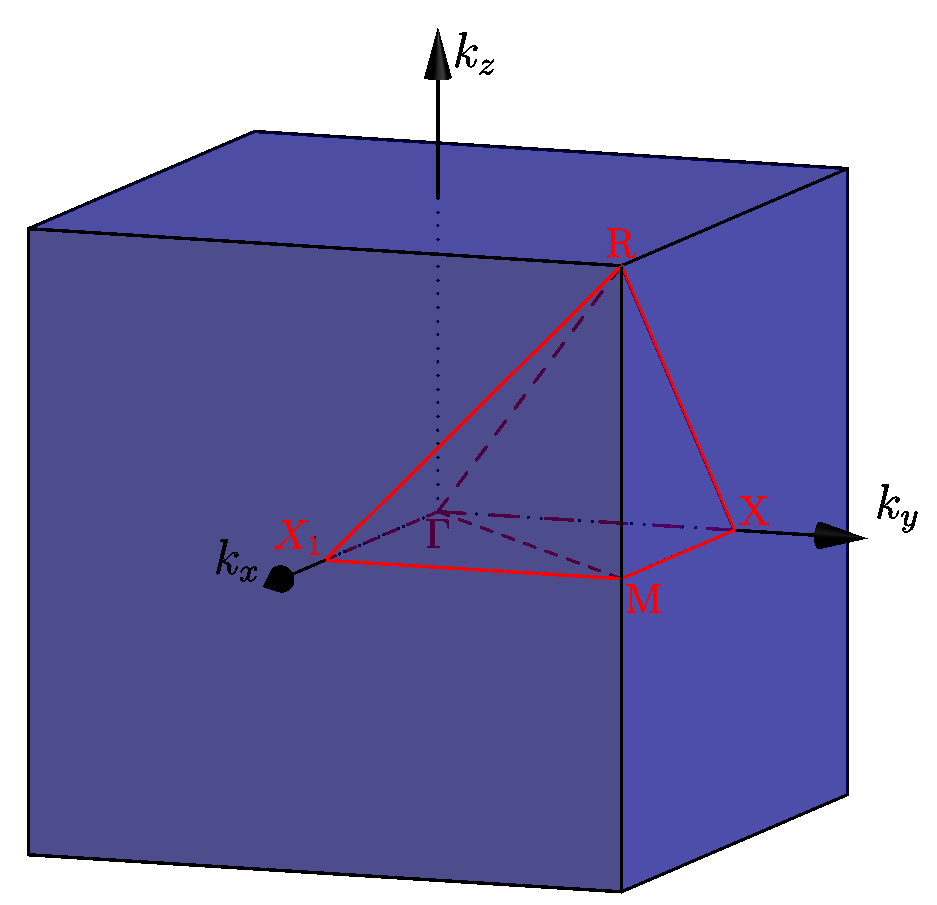
\includegraphics[width=7.5cm,angle=0]{images/cubic_bi.png}
\end{center}
\texttt{X$_1$} is available only with $\texttt{point\_label\_type='BI'}$.

\subsection{\texttt{ibrav=2}, face centered cubic lattice}
The primitive vectors of the direct lattice are:
\begin{eqnarray}
{\bf a}_1 &=& {a \over 2} (-1, 0, 1), \nonumber \\
{\bf a}_2 &=& {a \over 2} (0, 1, 1), \nonumber \\
{\bf a}_3 &=& {a \over 2} (-1, 1, 0), \nonumber
\nonumber
\end{eqnarray}
while the reciprocal lattice vectors are:
\begin{eqnarray}
{\bf b}_1 &=& {2\pi \over a} (-1, -1, 1), \nonumber \\
{\bf b}_2 &=& {2\pi \over a} (1, 1, 1), \nonumber \\
{\bf b}_3 &=& {2\pi \over a} (-1, 1, -1). \nonumber
\nonumber
\end{eqnarray}
The Brillouin zone is:
\begin{center}
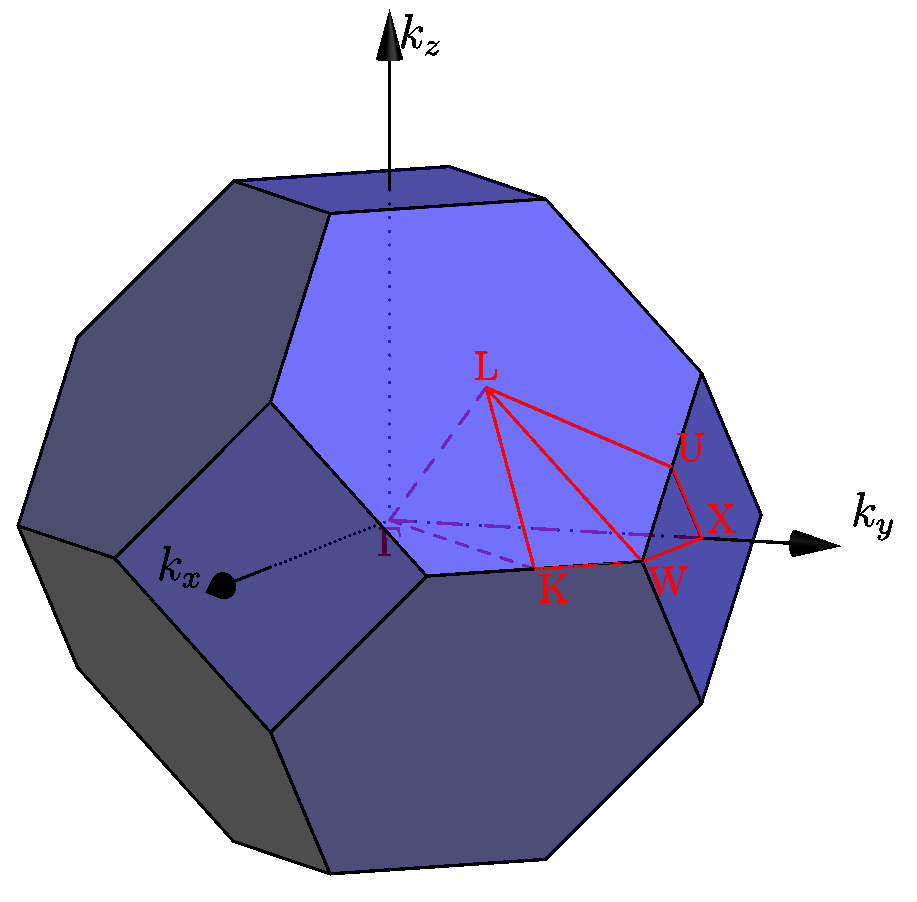
\includegraphics[width=7.5cm,angle=0]{images/fcc_sc.png} \hspace{1.cm}
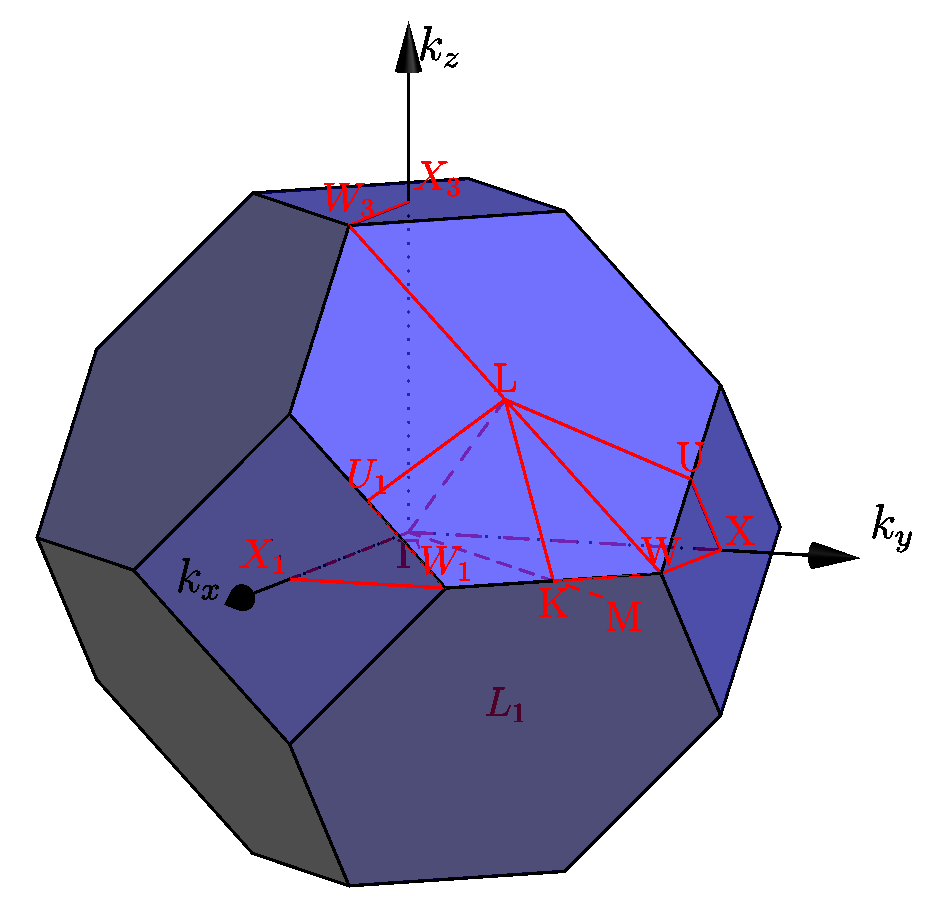
\includegraphics[width=7.5cm,angle=0]{images/fcc_bi.png}
\end{center}
Labels corresponding to $\texttt{point\_label\_type='SC'}$ and to
$\texttt{point\_label\_type='BI'}$ are shown on the left and on the right, 
respectively.

\subsection{\texttt{ibrav=3}, body centered cubic lattice}

The primitive vectors of the direct lattice are:
\begin{eqnarray}
{\bf a}_1 &=&{a \over 2} (1, 1, 1), \nonumber \\
{\bf a}_2 &=&{a \over 2} (-1, 1, 1), \nonumber \\
{\bf a}_3 &=&{a \over 2} (-1, -1, 1), \nonumber
\nonumber
\end{eqnarray}
while the reciprocal lattice vectors are:
\begin{eqnarray}
{\bf b}_1 &=&{2\pi \over a} (1, 0, 1), \nonumber \\
{\bf b}_2 &=&{2\pi \over a} (-1, 1, 0), \nonumber \\
{\bf b}_3 &=&{2\pi \over a} (0, -1, 1). \nonumber
\nonumber
\end{eqnarray}
\begin{center}
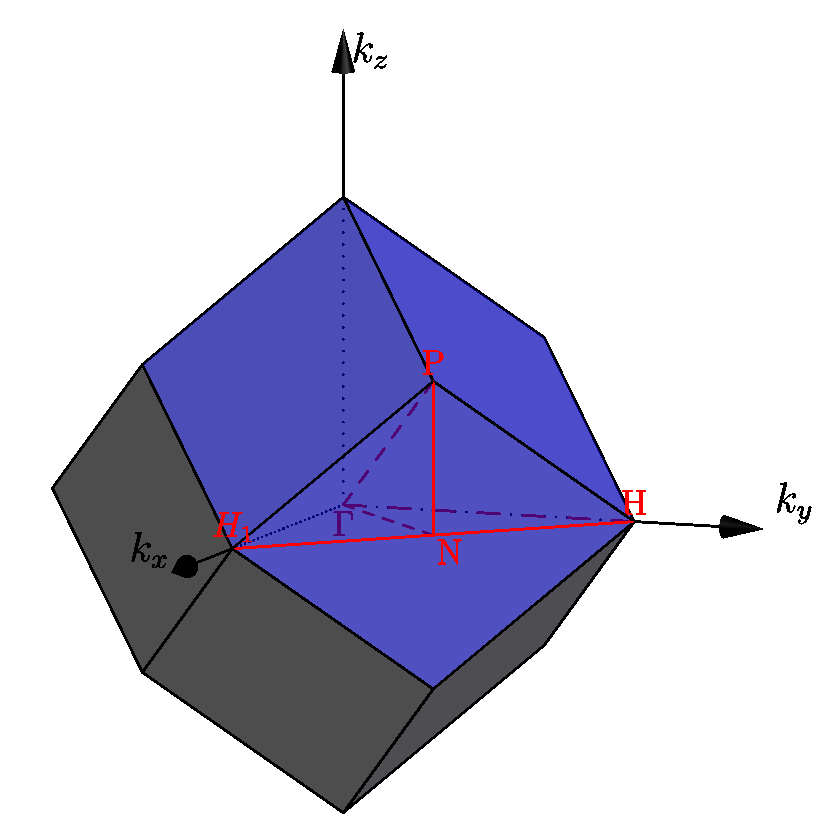
\includegraphics[width=7.5cm,angle=0]{images/bcc_bi.png}
\end{center}
\texttt{H$_1$} is available only with $\texttt{point\_label\_type='BI'}$.

\subsection{\texttt{ibrav=4}, hexagonal lattice}

The primitive vectors of the direct lattice are:
\begin{eqnarray}
{\bf a}_1 &=& a (1, 0, 0), \nonumber \\
{\bf a}_2 &=& a (-{1 \over 2}, {\sqrt{3} \over 2}, 0), \nonumber \\
{\bf a}_3 &=& a (0, 0, {c\over a}), \nonumber
\nonumber
\end{eqnarray}
while the reciprocal lattice vectors are:
\begin{eqnarray}
{\bf b}_1 &=& {2\pi \over a} (1, {1 \over \sqrt{3}}, 0), \nonumber \\
{\bf b}_2 &=& {2\pi \over a} (0, {2 \over \sqrt{3}}, 0), \nonumber \\
{\bf b}_3 &=& {2\pi \over a} (0, 0, {a\over c}). \nonumber
\nonumber
\end{eqnarray}
The BZ is:
\begin{center}
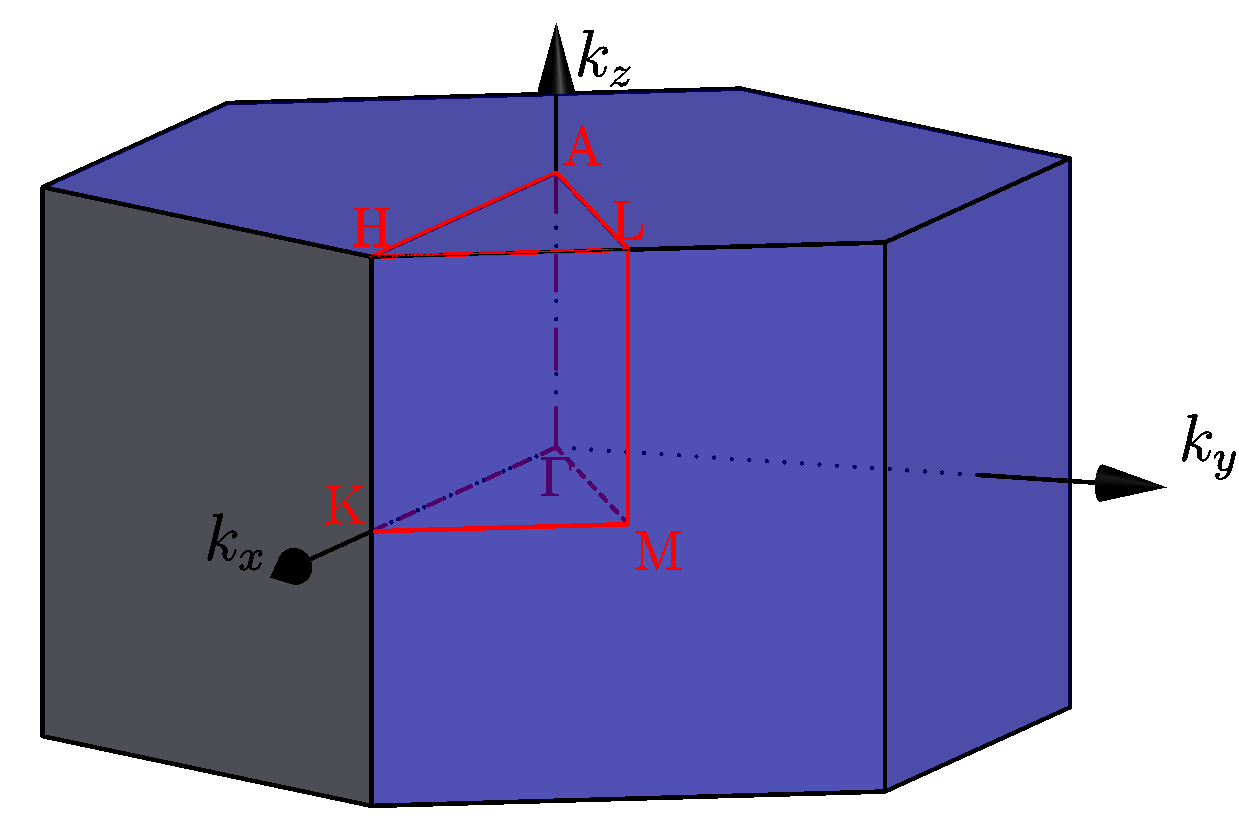
\includegraphics[width=7.5cm,angle=0]{images/hex.png}
\end{center}
The figure has been obtained with ${c/a}=1.4$.

\subsection{\texttt{ibrav=5}, trigonal lattice}

The primitive vectors of the direct lattice are:
\begin{eqnarray}
{\bf a}_1 &=& a ({\sqrt{3}\over 2}\sin{\theta}, -{1\over 2} \sin{\theta},
          \cos{\theta}), 
\nonumber \\
{\bf a}_2 &=& a (0, \sin{\theta}, \cos{\theta}), 
\nonumber \\
{\bf a}_3 &=& a (-{\sqrt{3}\over 2} \sin{\theta}, -{1\over 2} \sin{\theta},
         \cos{\theta}), 
\nonumber \\
\nonumber
\end{eqnarray}
while the reciprocal lattice vectors are:
\begin{eqnarray}
{\bf b}_1 &=& {2\pi \over a} ({1\over \sqrt{3} \sin{\theta}}, 
-{1 \over 3 \sin{\theta}}, {1\over 3 \cos{\theta}}), \nonumber \\
{\bf b}_2 &=& {2\pi \over a} (0, 
{2 \over 3 \sin{\theta}}, {1\over 3 \cos{\theta}}), \nonumber \\
{\bf b}_3 &=& {2\pi \over a} (-{1\over \sqrt{3} \sin{\theta}}, 
-{1 \over 3 \sin{\theta}}, {1\over 3 \cos{\theta}}), \nonumber \\
\end{eqnarray}
where $\sin{\theta}=\sqrt{2\over 3}\sqrt{1-\cos{\alpha}}$
and $\cos{\theta}=\sqrt{1\over 3}\sqrt{1 + 2 \cos{\alpha}}$ and $\alpha$
is the angle between any two primitive direct lattice vectors.
There are two possible shapes of the BZ, depending on the
value of the angle $\alpha$. For $\alpha < 90^\circ$ we
have:
\begin{center}
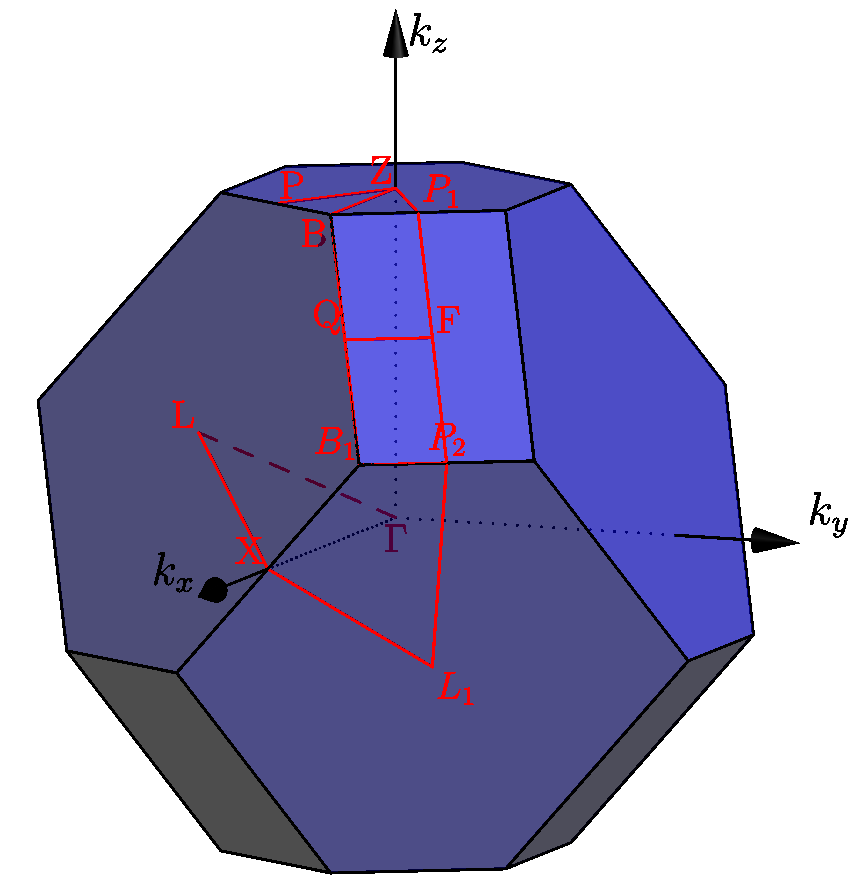
\includegraphics[width=7.5cm,angle=0]{images/tri_1.png}
\end{center}
The figure has been obtained with $\alpha=70^\circ$.
For $90^\circ < \alpha < 120^\circ$ we have:
\begin{center}
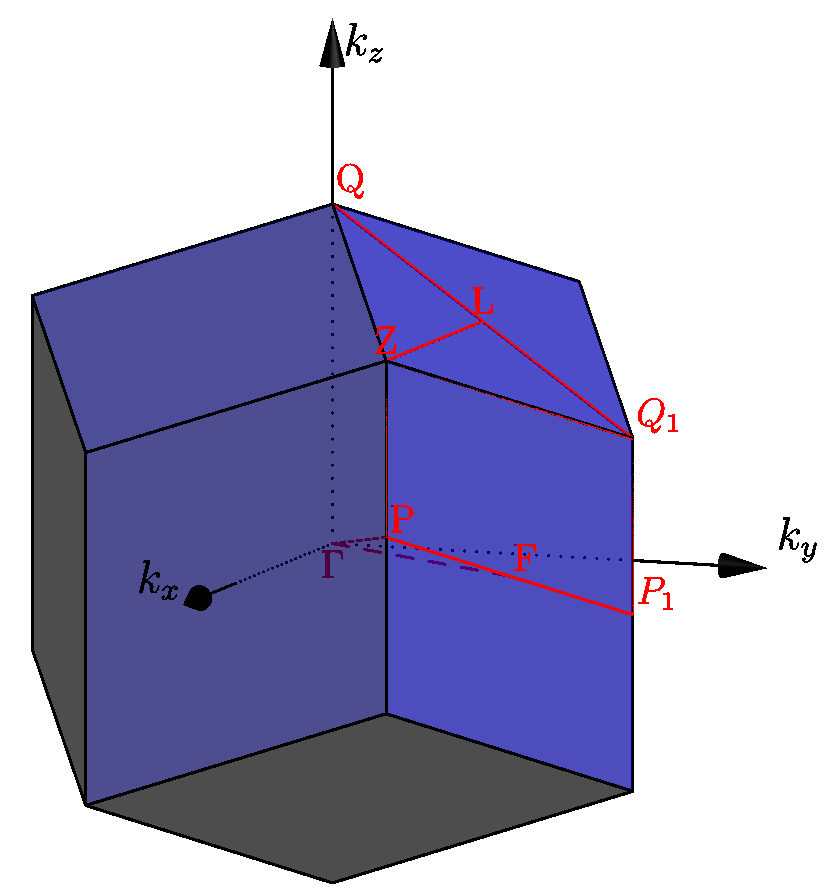
\includegraphics[width=7.5cm,angle=0]{images/tri_2.png}
\end{center}
The figure has been obtained with $\alpha=110^\circ$.

\subsection{\texttt{ibrav=6}, simple tetragonal lattice}
The primitive vectors of the direct lattice are:
\begin{eqnarray}
{\bf a}_1 &=& a (1, 0, 0), \nonumber \\
{\bf a}_2 &=& a (0, 1, 0), \nonumber \\
{\bf a}_3 &=& a (0, 0, {c\over a}), \nonumber
\nonumber
\end{eqnarray}
while the reciprocal lattice vectors are:
\begin{eqnarray}
{\bf b}_1 &=& {2\pi \over a} (1, 0, 0), \nonumber \\
{\bf b}_2 &=& {2\pi \over a} (0, 1, 0), \nonumber \\
{\bf b}_3 &=& {2\pi \over a} (0, 0, {a\over c}). \nonumber
\nonumber
\end{eqnarray}
\begin{center}
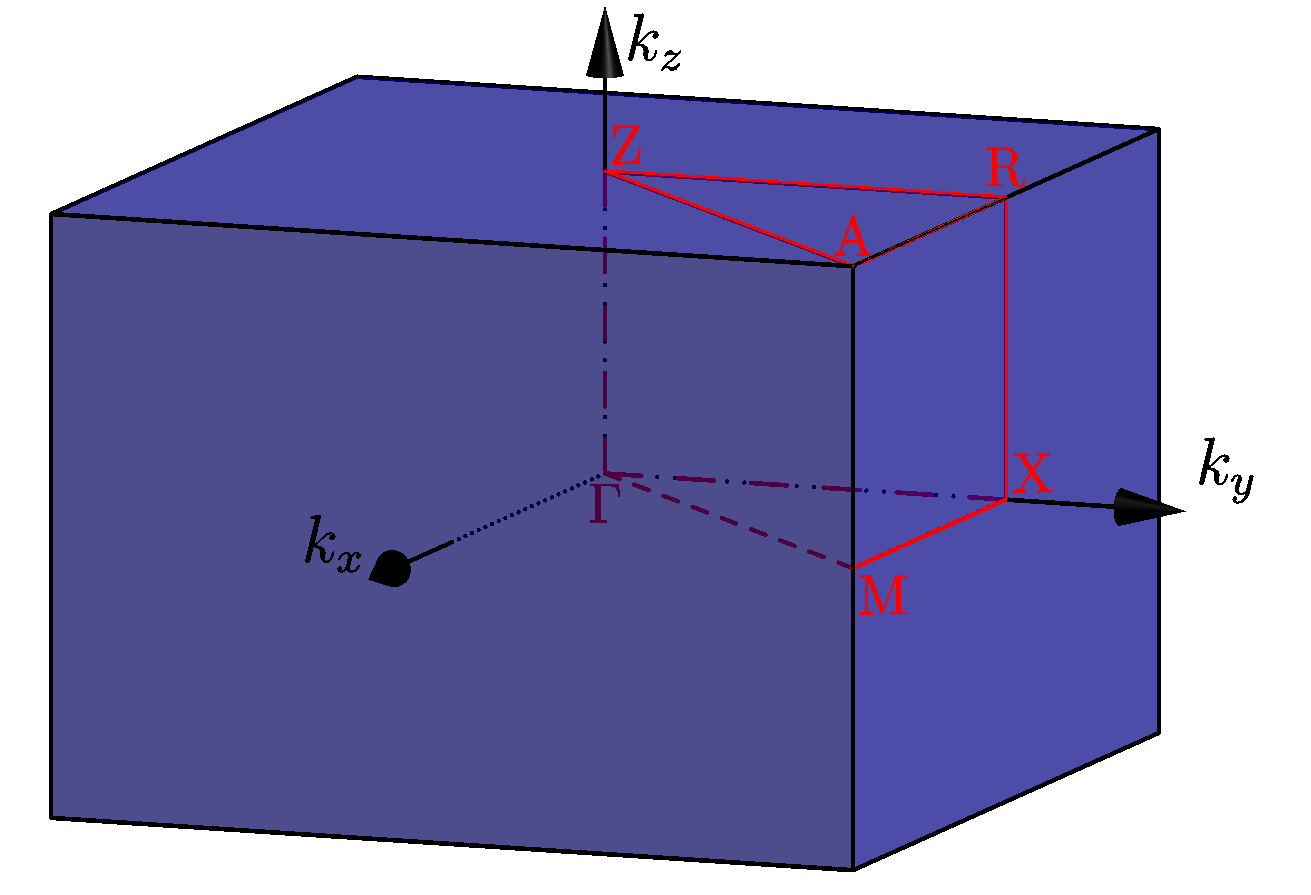
\includegraphics[width=7.5cm,angle=0]{images/st.png}
\end{center}
The figure has been obtained with $c/a=1.4$.

\subsection{\texttt{ibrav=7}, centered tetragonal lattice}
The primitive vectors of the direct lattice are:
\begin{eqnarray}
{\bf a}_1 &=& {a \over 2} (1, 1, {c\over a}), \nonumber \\
{\bf a}_2 &=& {a \over 2} (1, -1, {c\over a}), \nonumber \\
{\bf a}_3 &=& {a \over 2} (-1, -1, {c\over a}), \nonumber
\nonumber
\end{eqnarray}
while the reciprocal lattice vectors are:
\begin{eqnarray}
{\bf b}_1 &=& {2\pi \over a} (1, -1, 0), \nonumber \\
{\bf b}_2 &=& {2\pi \over a} (0, 1, {a\over c}), \nonumber \\
{\bf b}_3 &=& {2\pi \over a} (-1, 0, {a\over c}). \nonumber
\nonumber
\end{eqnarray}
In this case there are two different shapes of the BZ depending on the
$c/a$ ratio. For $c/a<1$ we have:
\begin{center}
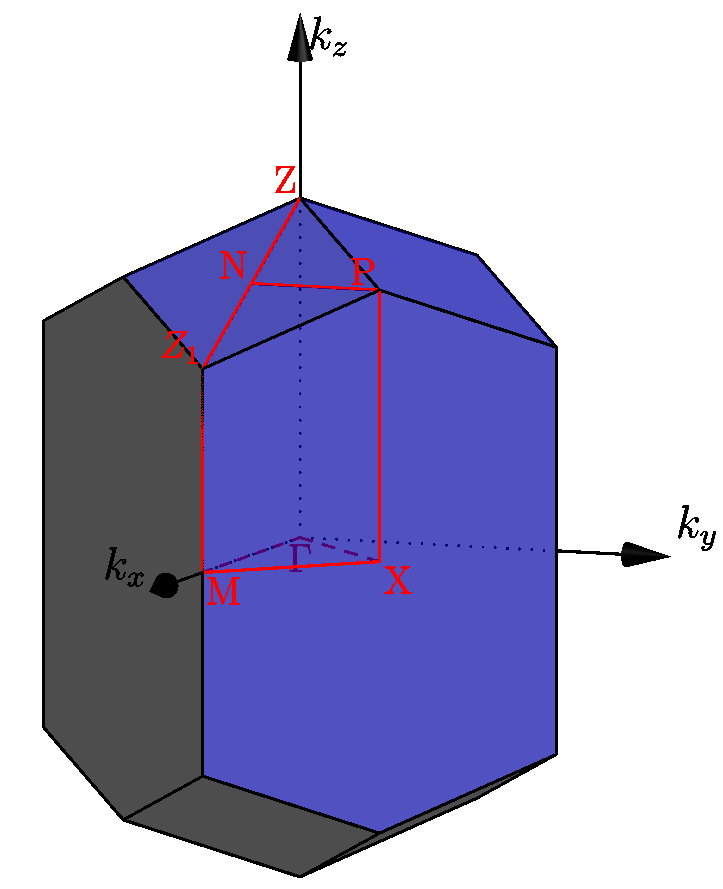
\includegraphics[width=7.5cm,angle=0]{images/stc1.png}
\end{center}
The figure has been obtained with $c/a=0.5$ ($a>c$). For $c/a>1$ we have:
\begin{center}
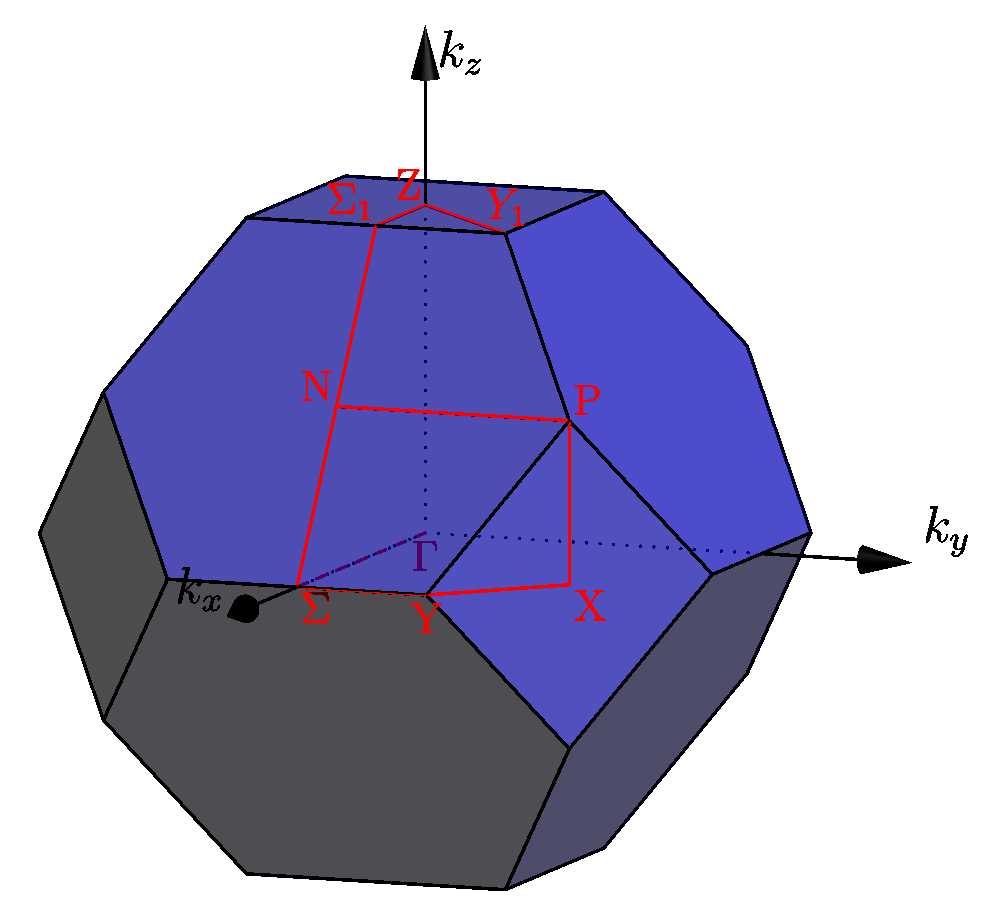
\includegraphics[width=7.5cm,angle=0]{images/stc2_sc.png} \hspace{1cm}
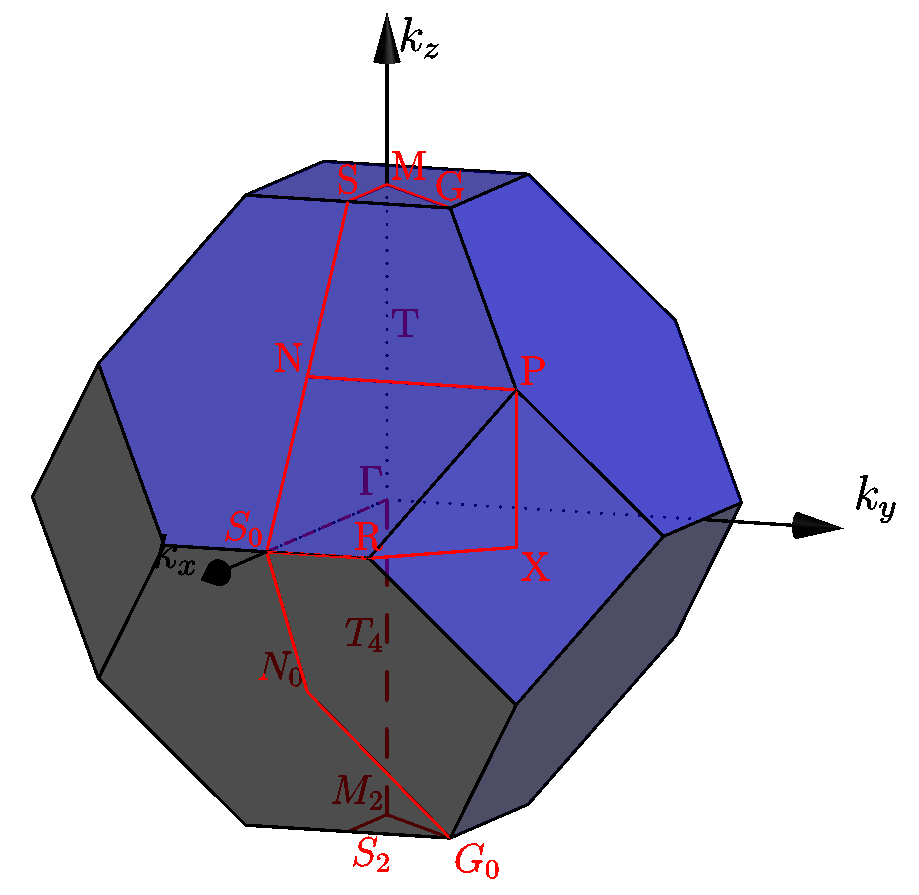
\includegraphics[width=7.5cm,angle=0]{images/stc2.png}
\end{center}
The figure has been obtained with $c/a=1.4$ ($a<c$).
Labels corresponding to $\texttt{point\_label\_type='SC'}$ are shown on the left,
those corresponding to $\texttt{point\_label\_type='BI'}$ on the right.

\subsection{\texttt{ibrav=8}, simple orthorhombic lattice}
The primitive vectors of the direct lattice are:
\begin{eqnarray}
{\bf a}_1 &=& a (1, 0, 0), \nonumber \\
{\bf a}_2 &=& a (0, {b\over a}, 0), \nonumber \\
{\bf a}_3 &=& a (0, 0, {c\over a}), \nonumber
\nonumber
\end{eqnarray}
while the reciprocal lattice vectors are:
\begin{eqnarray}
{\bf b}_1 &=& {2\pi \over a} (1, 0, 0), \nonumber \\
{\bf b}_2 &=& {2\pi \over a} (0, {a\over b}, 0), \nonumber \\
{\bf b}_3 &=& {2\pi \over a} (0, 0, {a\over c}). \nonumber
\nonumber
\end{eqnarray}
\begin{center}
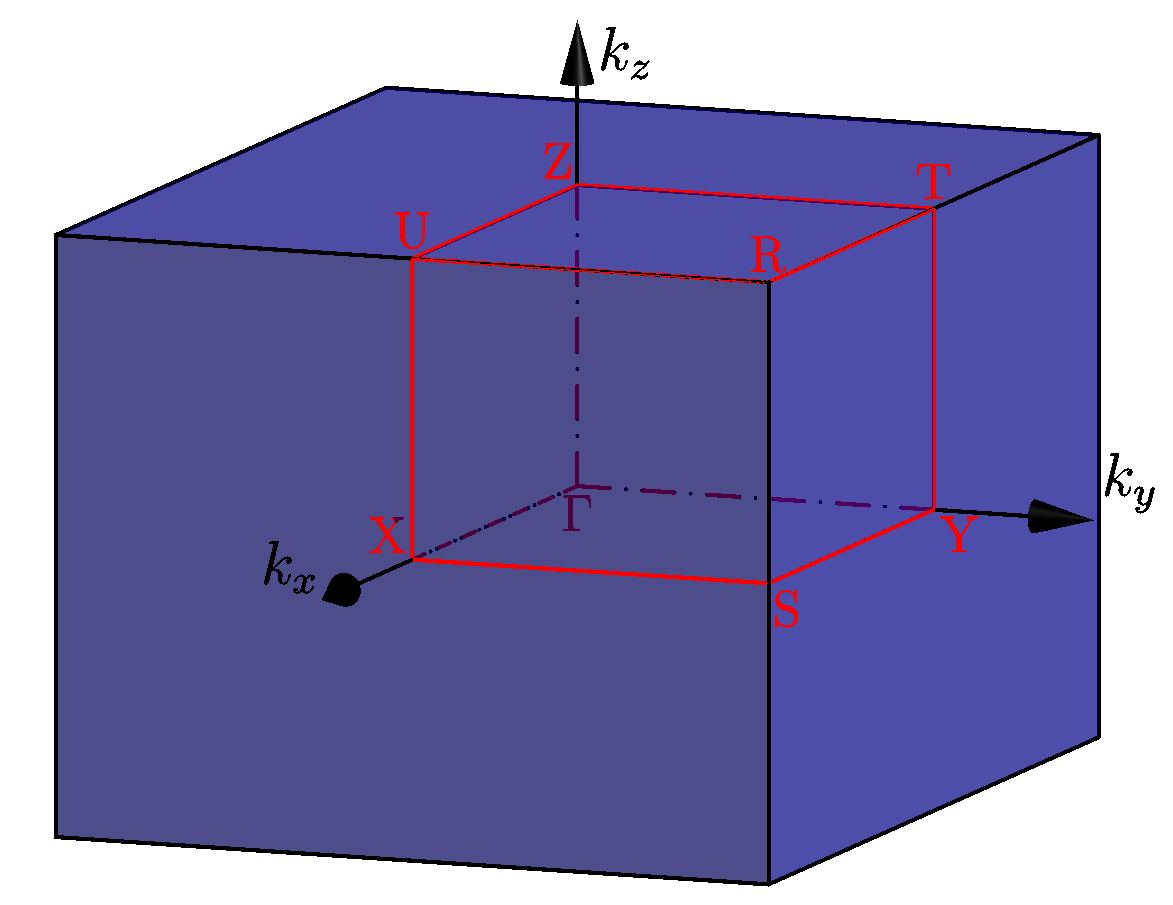
\includegraphics[width=7.5cm,angle=0]{images/so.png}
\end{center}
The figure has been obtained with $b/a=1.2$ and $c/a=1.5$.

\subsection{\texttt{ibrav=9}, one-face centered orthorhombic lattice}
The direct lattice vectors are:
\begin{eqnarray}
{\bf a}_1 &=& {a \over 2} (1, {b \over a}, 0), \nonumber \\
{\bf a}_2 &=& {a \over 2} (-1, {b \over a}, 0), \nonumber \\
{\bf a}_3 &=& a  (0, 0, {c \over a}), \nonumber
\nonumber
\end{eqnarray}
while the reciprocal lattice vectors are
\begin{eqnarray}
{\bf b}_1 &=& {2\pi \over a} (1, {a \over b}, 0), \nonumber \\
{\bf b}_2 &=& {2\pi \over a} (-1, {a \over b}, 0), \nonumber \\
{\bf b}_3 &=& {2\pi \over a} (0, 0, {a \over c}). \nonumber
\nonumber
\end{eqnarray}
There is one shape that can have two orientations depending on the
ratio between of $a$ and $b$:
\begin{center}
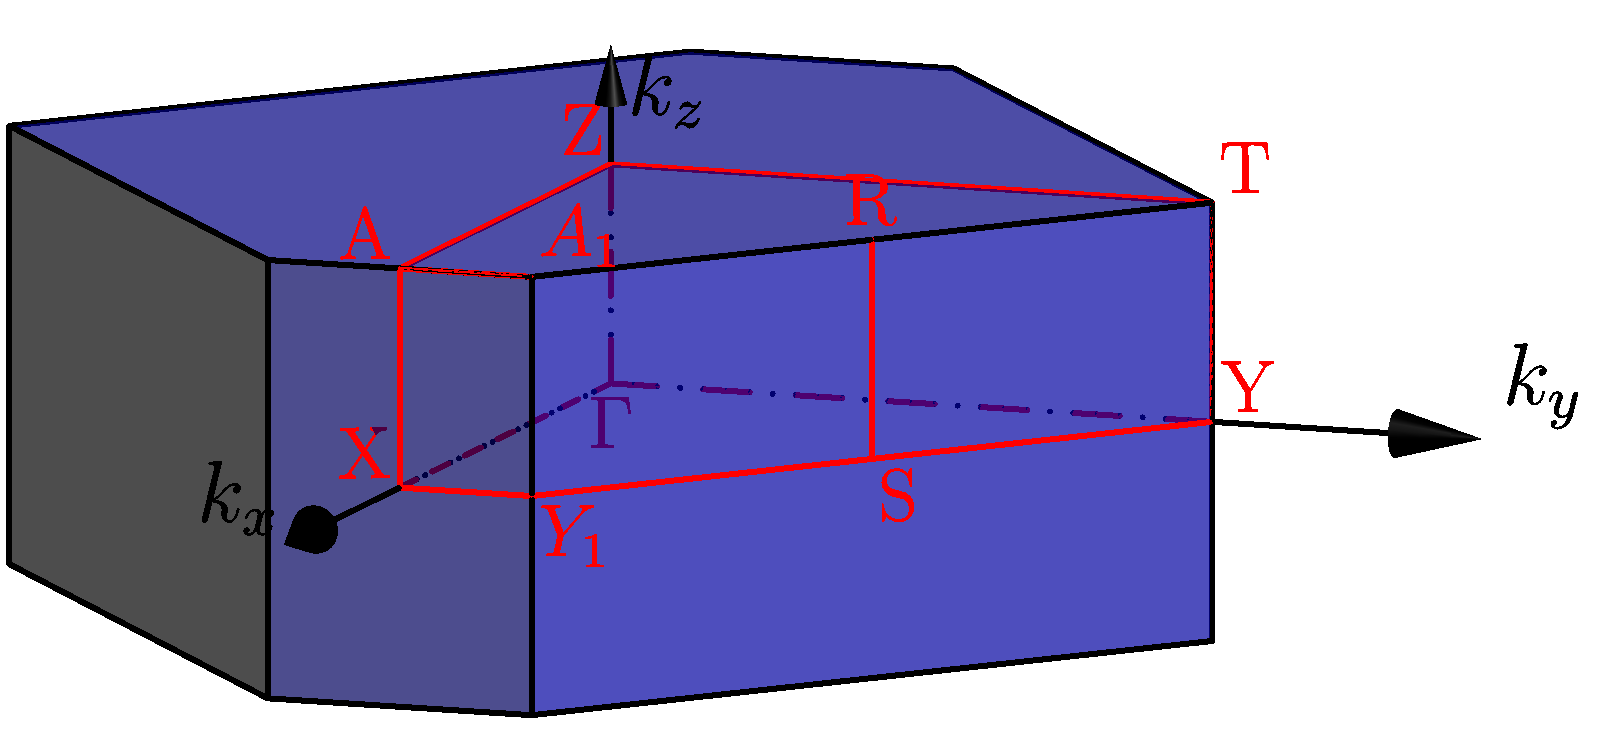
\includegraphics[width=7.5cm,angle=0]{images/ofco_2.png} \hspace{1cm}
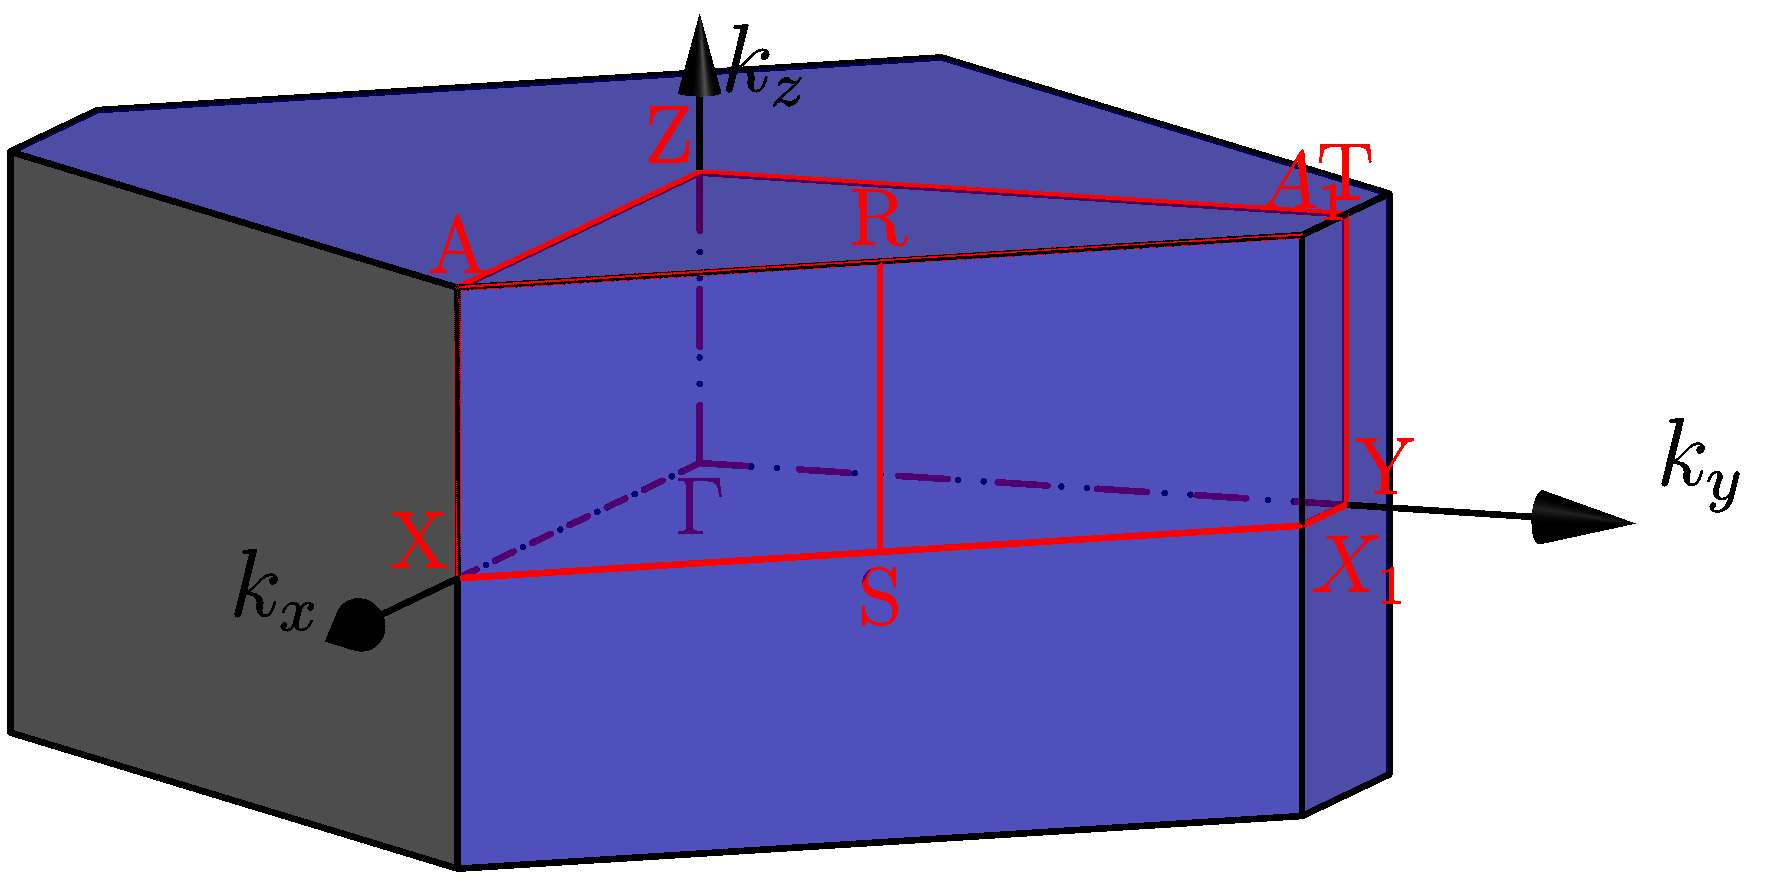
\includegraphics[width=6.5cm,angle=0]{images/ofco_1.png}
\end{center}
The figures have been obtained with $b/a=0.8$ and $c/a=1.4$ (left part $b<a$) 
and $b/a=1.2$ and $c/a=1.4$ (right part $b>a$).

\subsection{\texttt{ibrav=10}, face centered orthorhombic lattice}
The direct lattice vectors are:
\begin{eqnarray}
{\bf a}_1 &=& {a \over 2} (1, 0, {c \over a}), \nonumber \\
{\bf a}_2 &=& {a \over 2} (1, {b \over a}, 0), \nonumber \\
{\bf a}_3 &=& {a \over 2} (0, {b \over a}, {c \over a}). \nonumber
\nonumber
\end{eqnarray}
while the reciprocal lattice vectors are
\begin{eqnarray}
{\bf b}_1 &=& {2\pi \over a} (1, -{a \over b}, {a \over c}), \nonumber \\
{\bf b}_2 &=& {2\pi \over a} (1, {a \over b}, -{a \over c}), \nonumber \\
{\bf b}_3 &=& {2\pi \over a} (-1, {a \over b}, {a \over c}). \nonumber
\nonumber
\end{eqnarray}
In this case there are three different shapes 
that can be rotated in different ways depending on the relative
sizes of $a$, $b$, and $c$. 
If $a$ is the shortest side, there are three different shapes according
to 
\begin{equation}
{1\over a^2} \lesseqqgtr
{1\over b^2} + {1\over c^2},
\label{uno}
\end{equation}
if $b$ is the shortest side there are three different shapes according to 
\begin{equation}
{1\over b^2} \lesseqqgtr {1\over a^2} + {1\over c^2},
\label{due}
\end{equation}
and if $c$ is the shortest side there are
three different shapes according to 
\begin{equation}
{1\over c^2} \lesseqqgtr {1\over a^2} 
+ {1\over b^2}.
\label{tre}
\end{equation}
For each case there are two possibilities. If $a$
is the shortest side, we can have $b<c$ or $b>c$, if $b$ is
the shortest side, we can have $a<c$ or $a>c$, and finally
if $c$ is the shortest side we can have $a<b$ or $a>b$. In total we
have $18$ distinct cases. Not all cases give different BZ.
All the cases with the $<$ sign in Eqs.~\ref{uno}, \ref{due}, \ref{tre} give
the same shape of the BZ that differ for the relative sizes of the faces. 
All the cases with the $>$ sign in Eqs.~\ref{uno}, \ref{due}, \ref{tre} give 
the same shape with faces of different sizes and oriented in different ways. 
Finally the particular case with the $=$ sign in Eqs.~\ref{uno}, 
\ref{due}, \ref{tre} give another shape 
with faces of different size and different orientations. 
We show all the 18 possibilities and the labels used in each case.

We start with the case in which $a$ is the shortest side and show on the
left the case $b<c$ and on the right the case $b>c$. 
The first possibility is that ${1\over a^2} <
{1\over b^2} + {1\over c^2}$:
\begin{center}
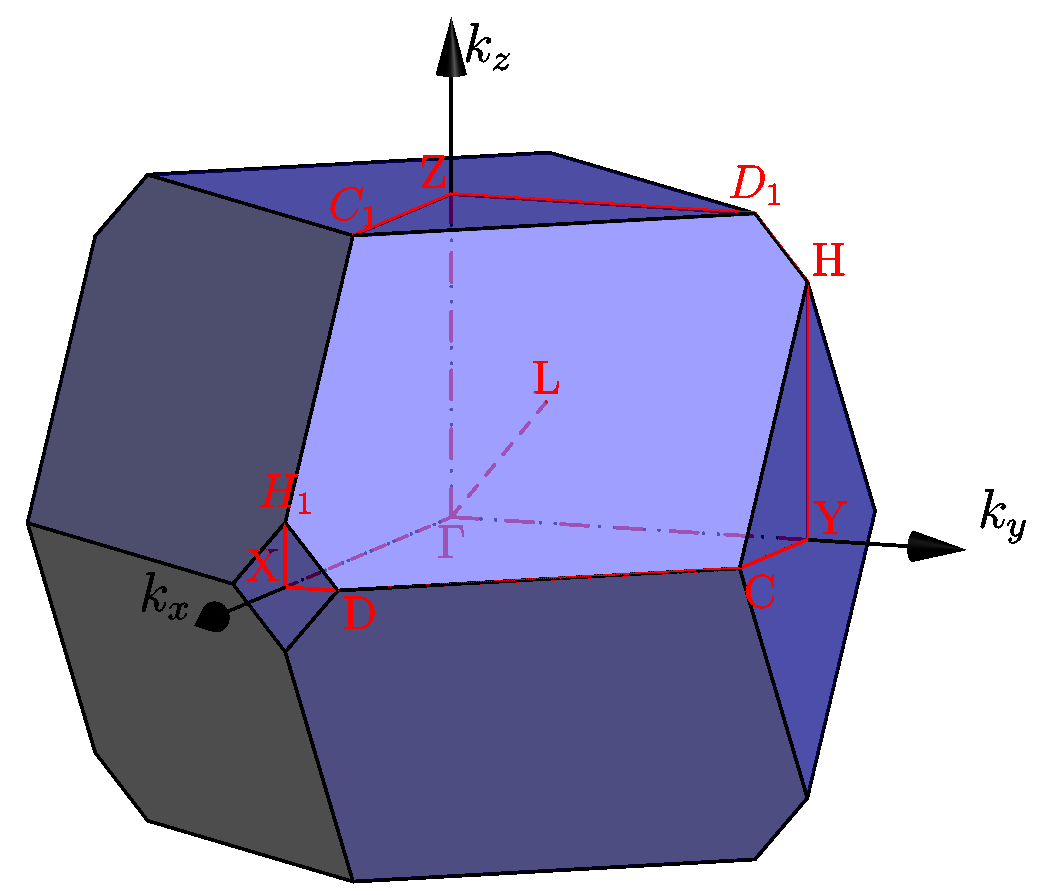
\includegraphics[width=7.5cm,angle=0]{images/ofc_1.png} \hspace{1cm}
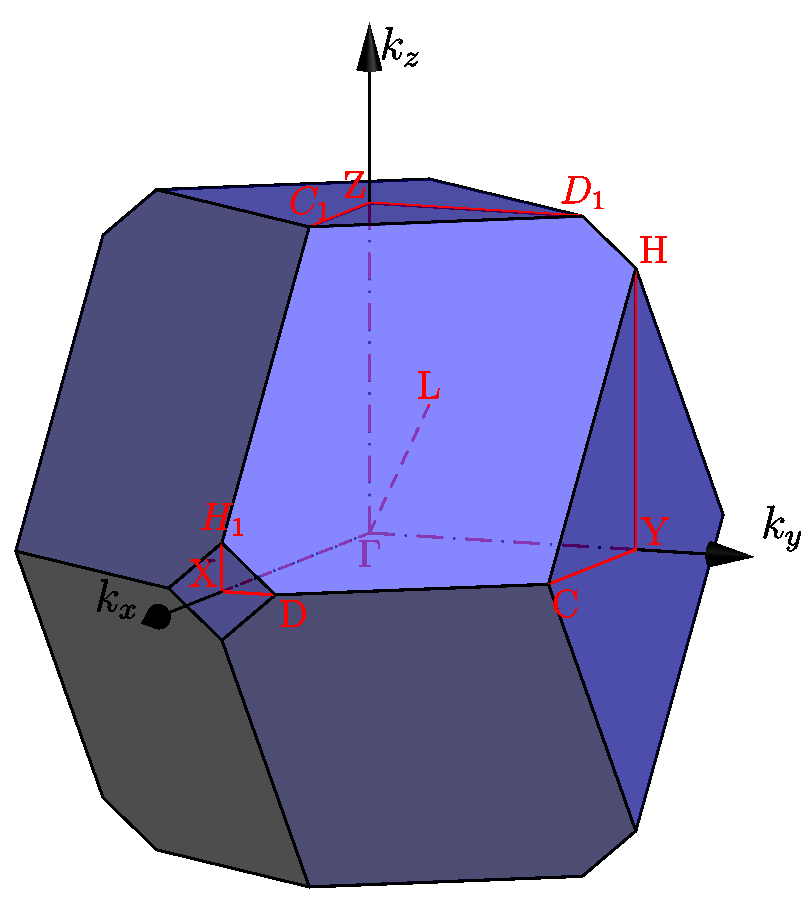
\includegraphics[width=6.5cm,angle=0]{images/ofc_2.png} 
\end{center}
The figures have been obtained with $b/a=1.2$ and $c/a=1.4$ (left part $b<c$),
and with $b/a=1.4$ and $c/a=1.2$ (right part $b>c$).

The second possibility is that ${1\over a^2} =
{1\over b^2} + {1\over c^2}$:
\begin{center}
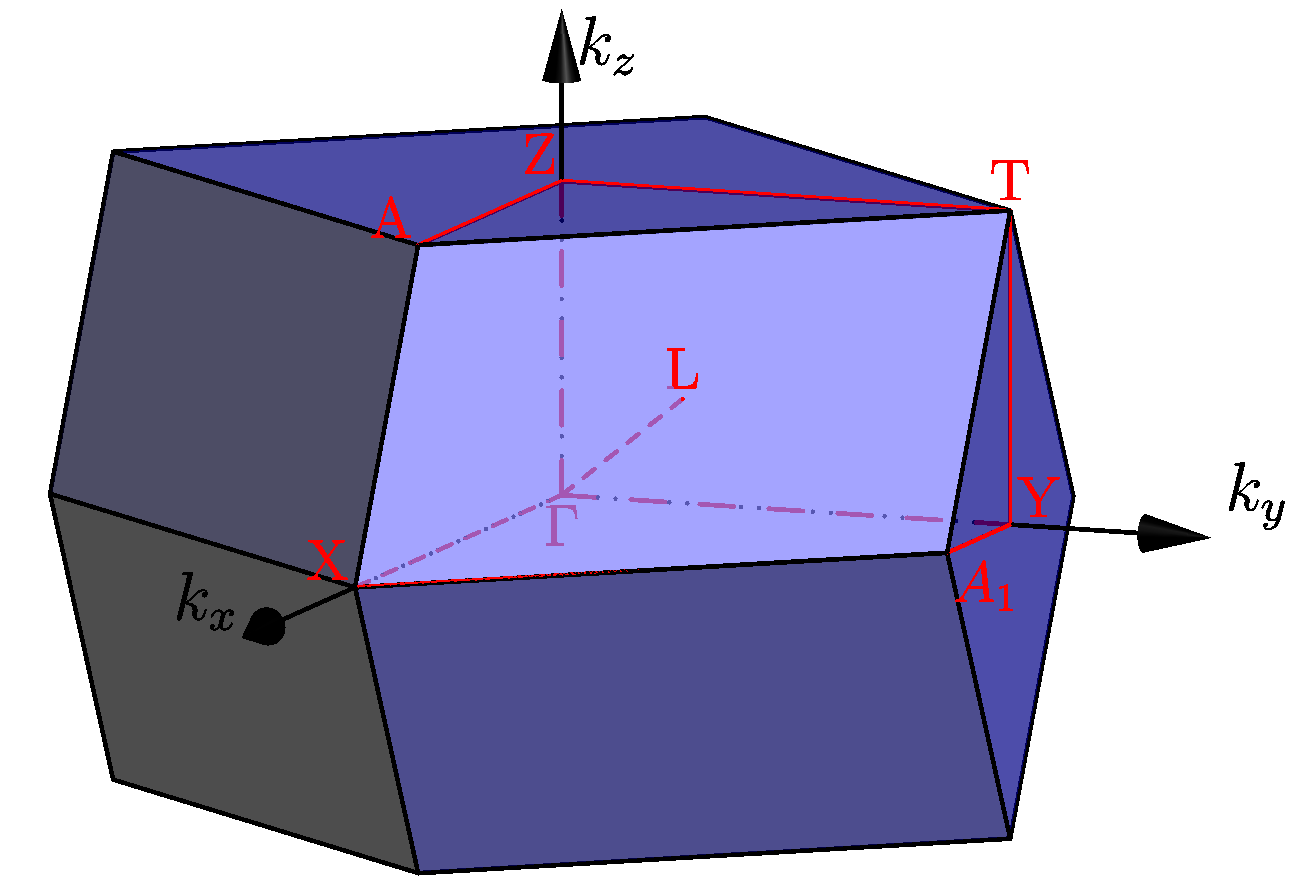
\includegraphics[width=7.5cm,angle=0]{images/ofc_13.png} \hspace{1cm}
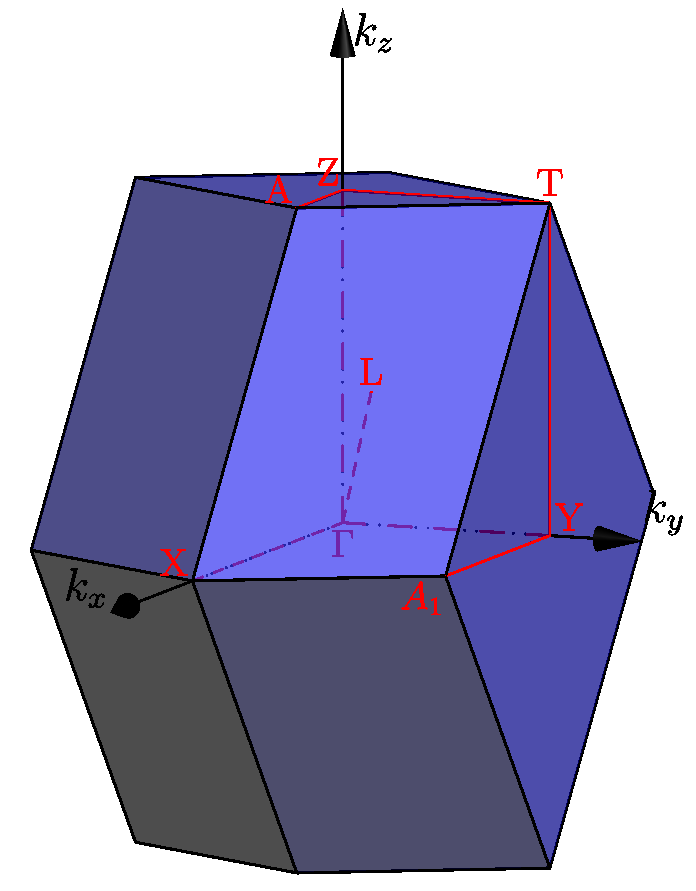
\includegraphics[width=5.5cm,angle=0]{images/ofc_14.png} 
\end{center}
The figures have been obtained with $b/a=1.2$ and $c/a=1.80906807$ 
(left part $b<c$) and with $b/a=1.80906807$ and $c/a=1.2$ (right part $b>c$).

The third possibility is that ${1 \over a^2} > {1\over b^2} + {1\over c^2}$:
\begin{center}
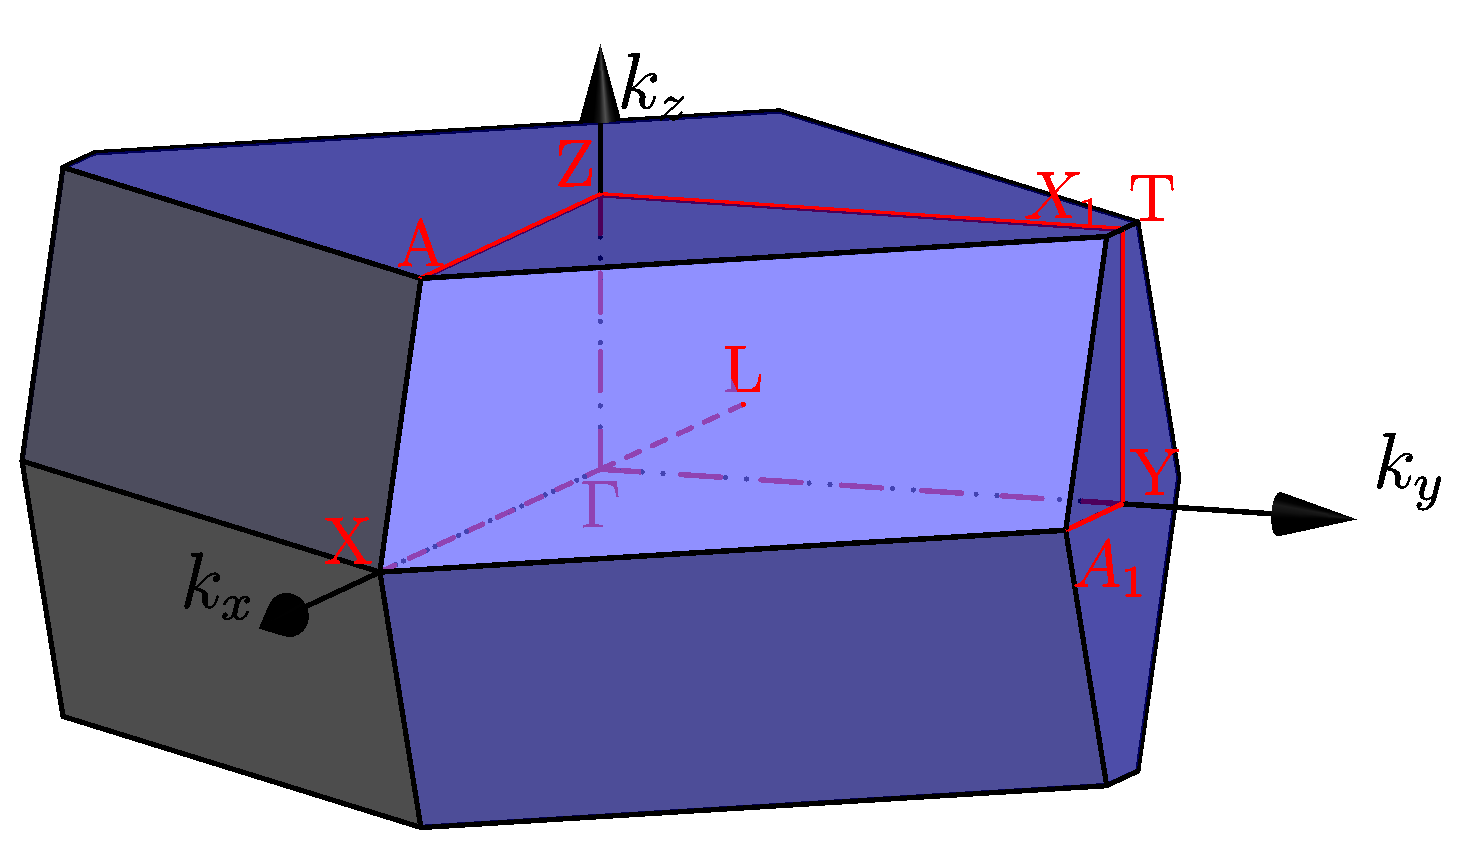
\includegraphics[width=6.5cm,angle=0]{images/ofc_7.png} \hspace{1cm}
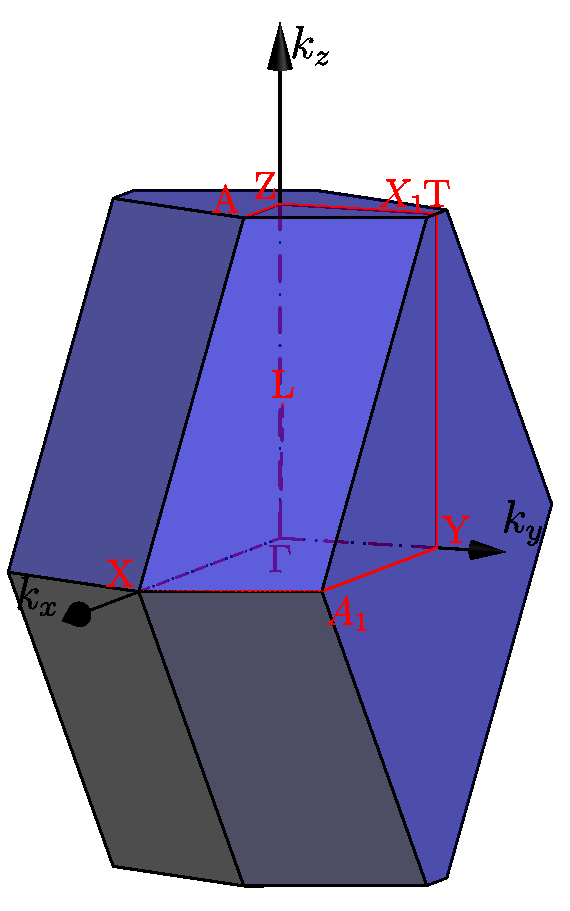
\includegraphics[width=4.0cm,angle=0]{images/ofc_8.png} 
\end{center}
The figures have been obtained with $b/a=1.2$ and $c/a=2.4$ (left part $b<c$), 
and with $b/a=2.4$ and $c/a=1.2$ (right part $b>c$).

Then we consider the cases in which $b$ is the shortest side and show
on the left the case in which $a<c$ and on the right the case $a>c$. 

We have the same three possibilities as before. The first possibility
is that ${1 \over b^2} < {1\over a^2} + {1\over c^2}$: 
\begin{center}
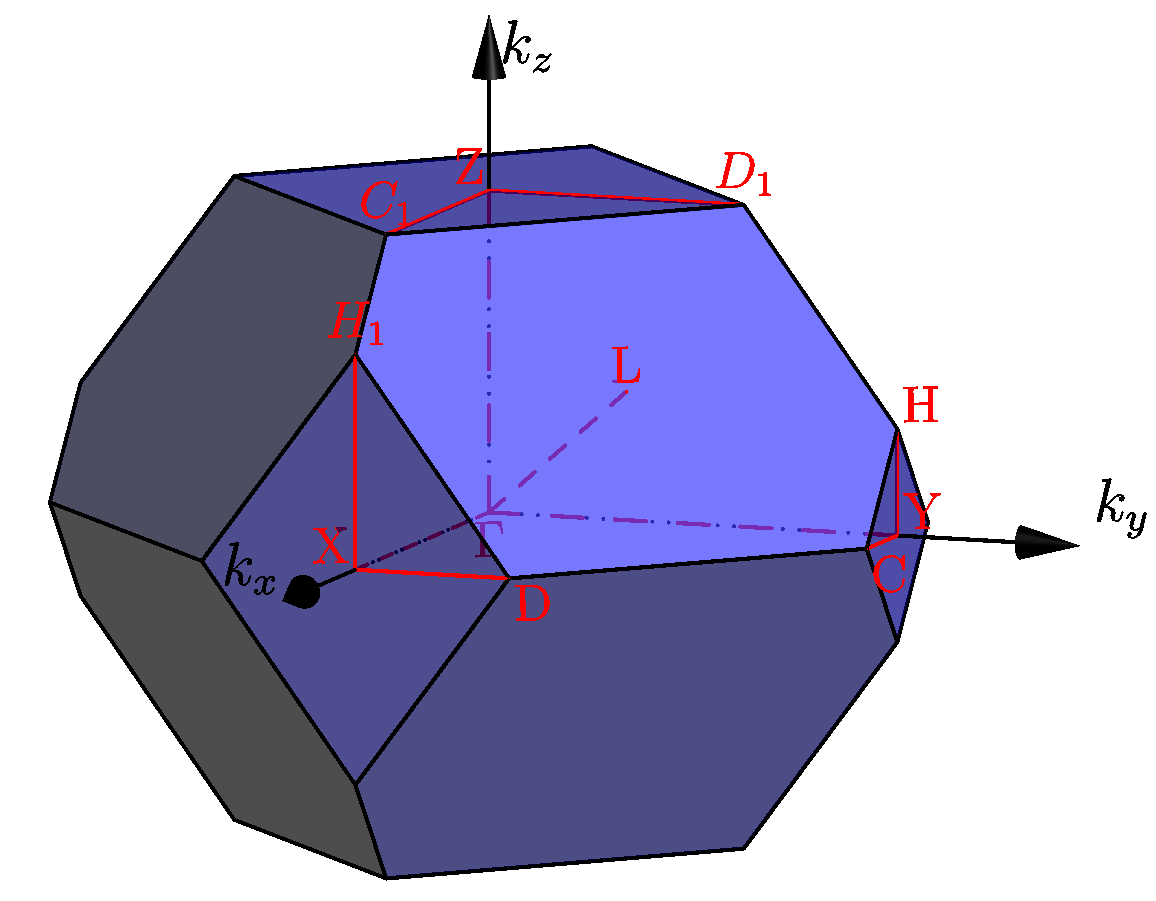
\includegraphics[width=7.5cm,angle=0]{images/ofc_3.png} \hspace{1cm}
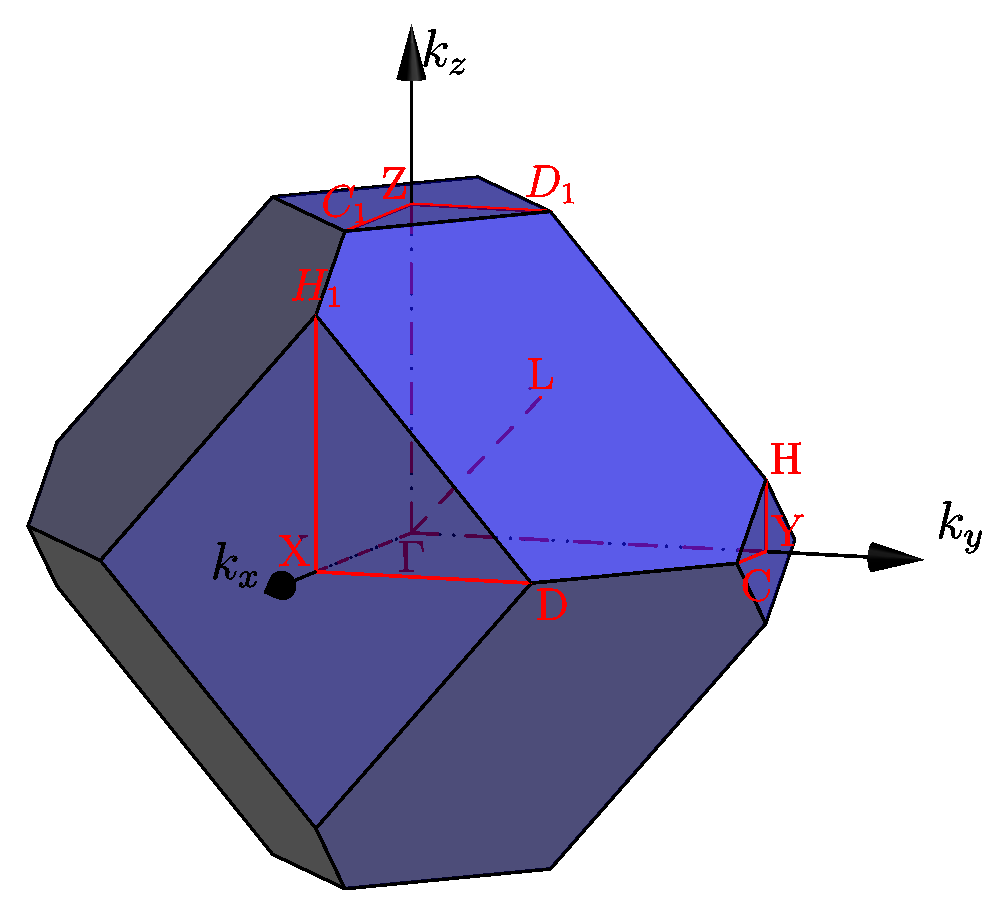
\includegraphics[width=7.5cm,angle=0]{images/ofc_4.png} \hspace{1cm}
\end{center}
The figures have been obtained with $b/a=0.9$ and $c/a=1.2$ 
(left part $a<c$) and $b/a=0.75$ and $c/a=0.95$ (right part $a>c$).

The second possibility is that ${1 \over b^2}={1\over a^2} + {1\over c^2}$:
\begin{center}
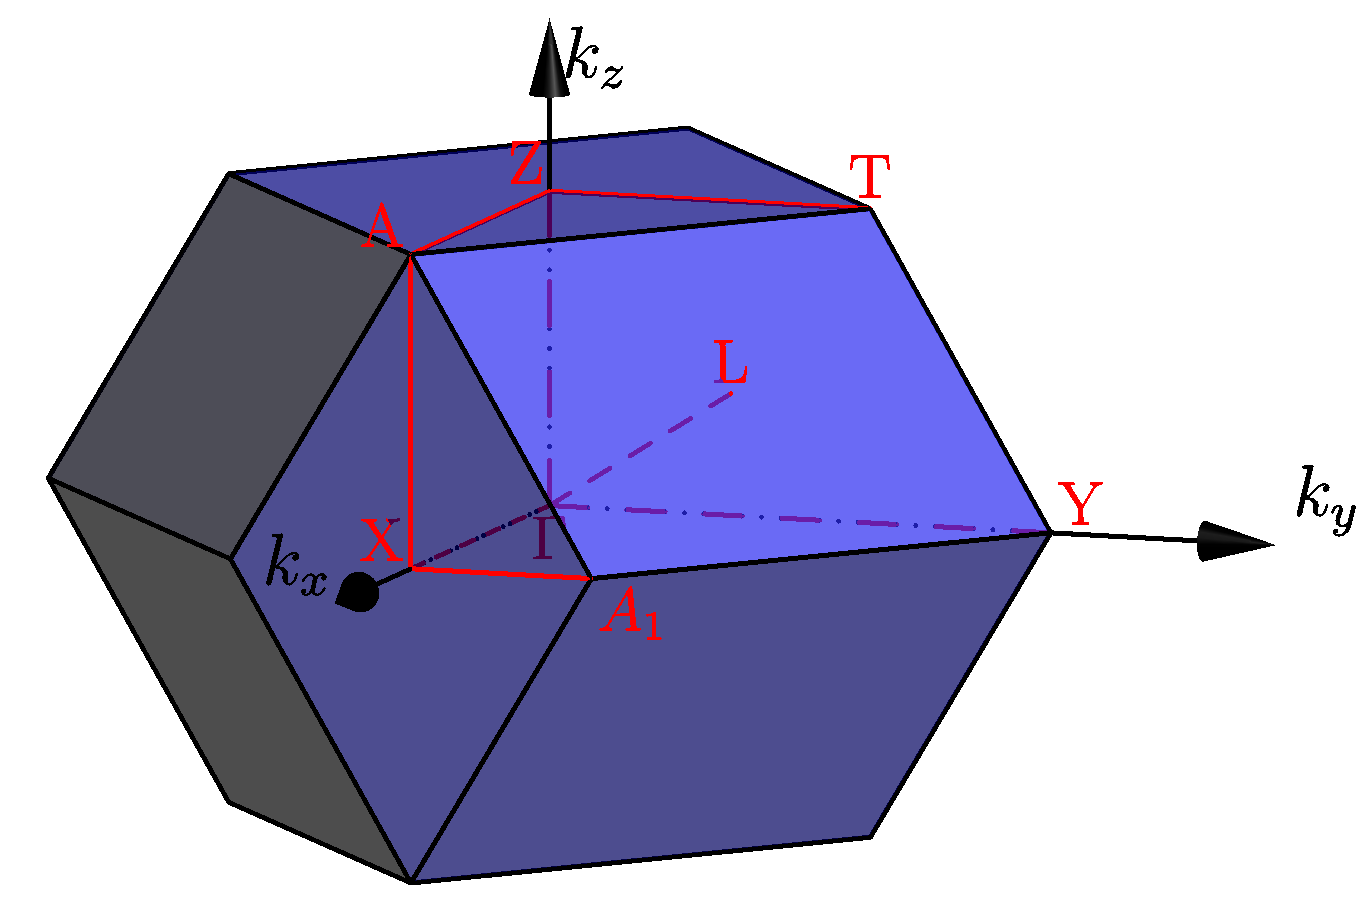
\includegraphics[width=7.5cm,angle=0]{images/ofc_15.png} \hspace{1cm}
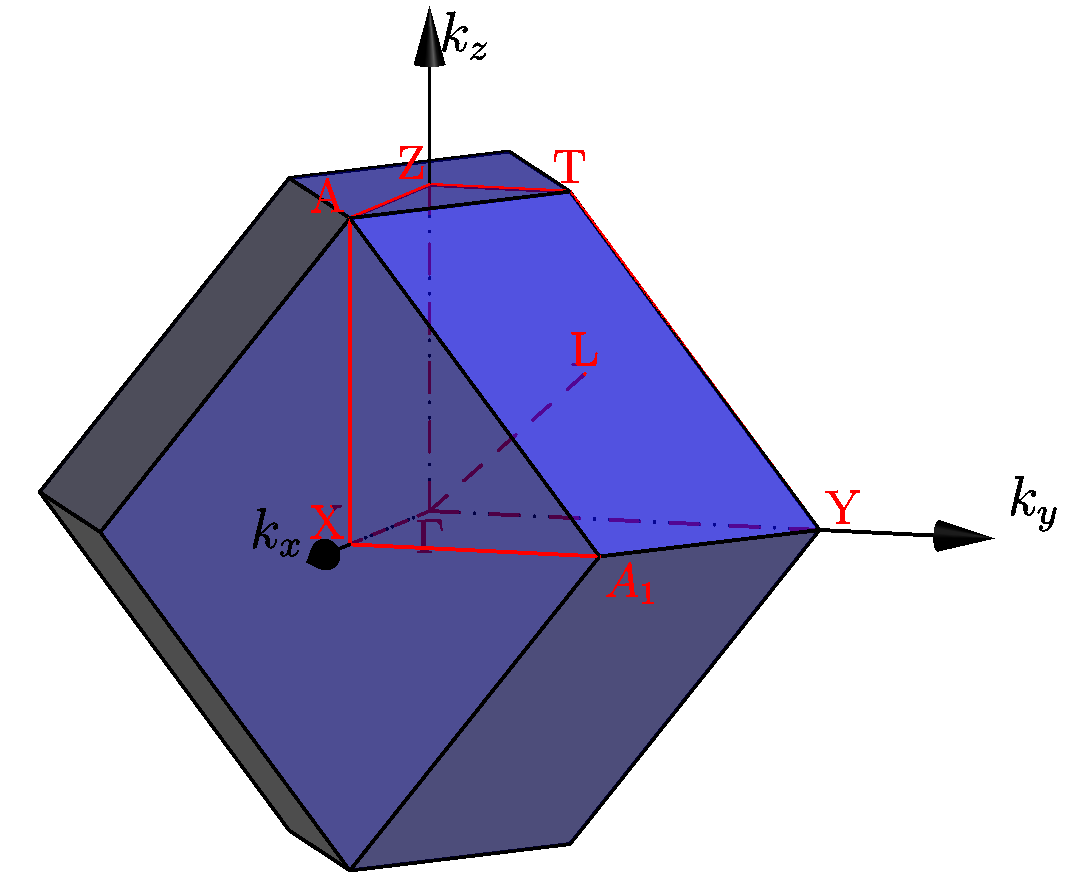
\includegraphics[width=7.5cm,angle=0]{images/ofc_16.png} 
\end{center}
The figures have been obtained with $b/a=0.8$ and $c/a=1.33333333333$ (left
part $a<c$), and $b/a=0.6$ and $c/a=0.75$ (right part $a>c$).

The third possibility is than ${1\over b^2}>{1\over a^2} + {1\over c^2}$:
\begin{center}
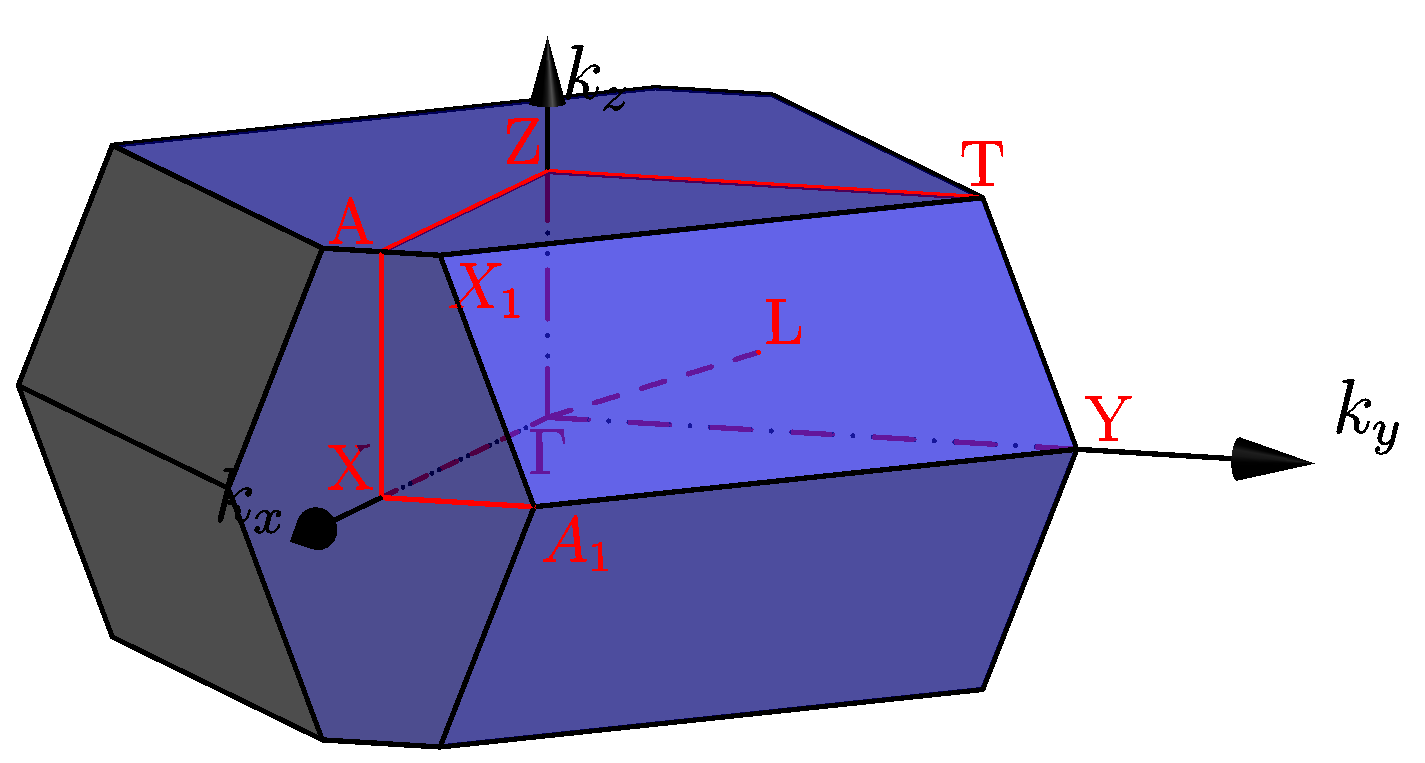
\includegraphics[width=7.5cm,angle=0]{images/ofc_9.png} \hspace{1cm}
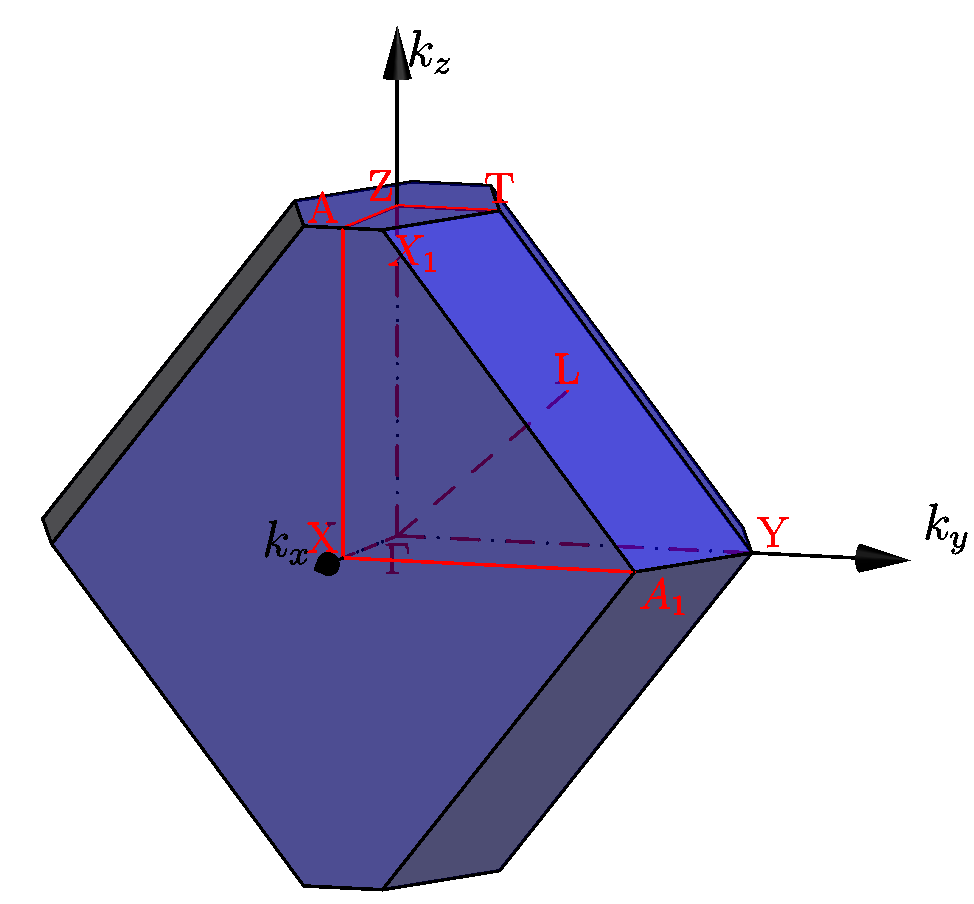
\includegraphics[width=7.5cm,angle=0]{images/ofc_10.png} 
\end{center}
The figures have been obtained with $b/a=0.8$ and $c/a=2.0$ (left part $a<c$),
and with $b/a=0.4$ and $c/a=0.5$ (right part $a>c$).

Finally we consider the case in which $c$ is the shortest side and show on
the left the case in which $a<b$ and on the right the case in which $a>b$. 

The first possibility is that ${1\over c^2}<{1\over a^2} + {1\over b^2}$:
\begin{center}
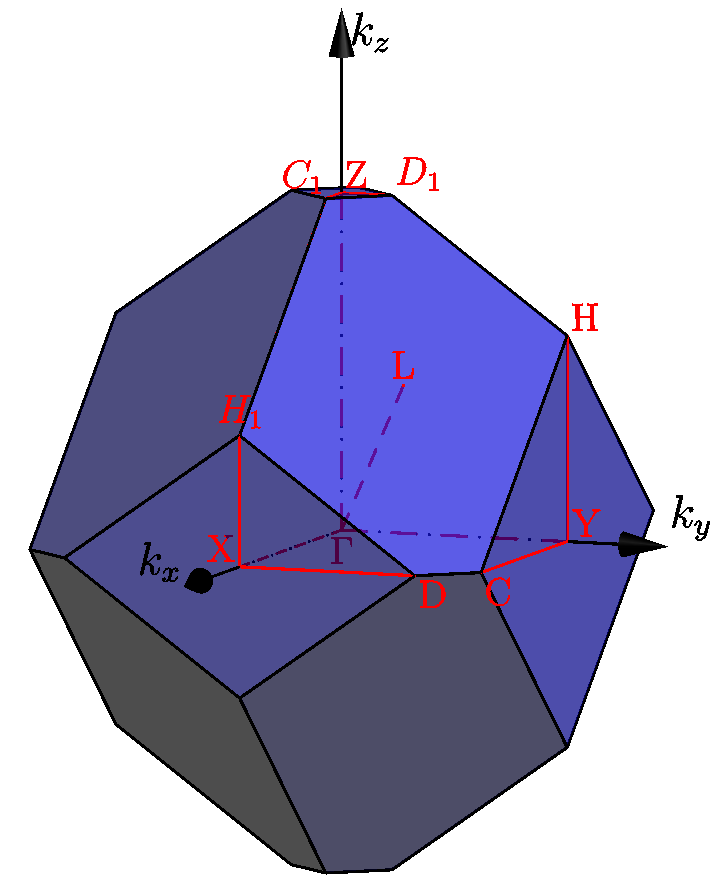
\includegraphics[width=6.5cm,angle=0]{images/ofc_5.png} \hspace{1cm}
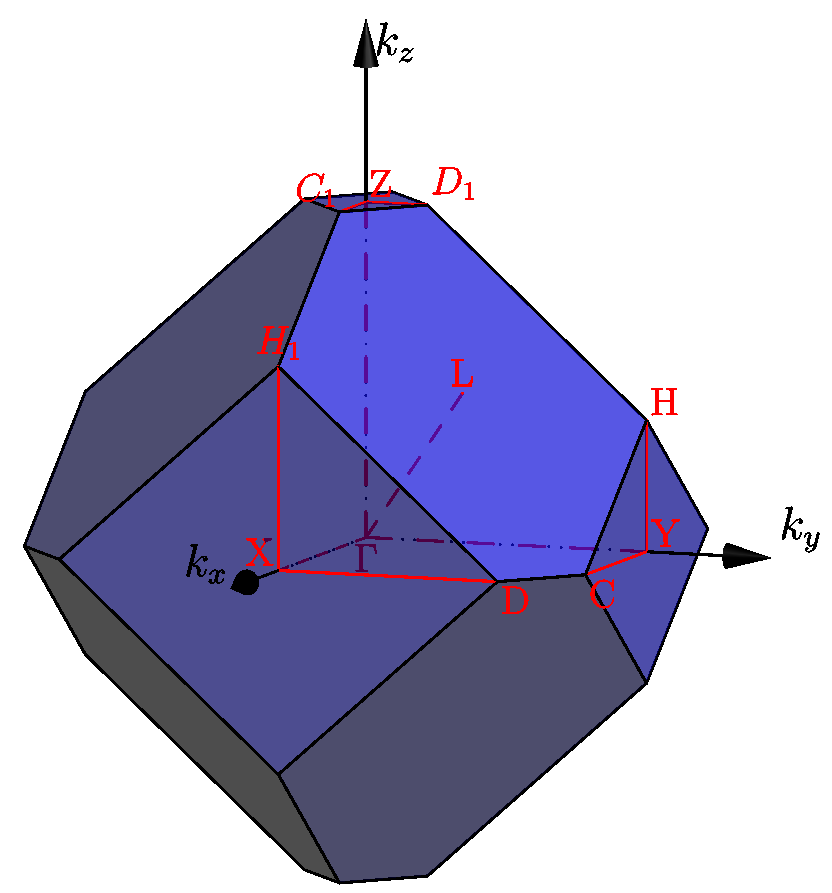
\includegraphics[width=7.5cm,angle=0]{images/ofc_6.png} 
\end{center}
The figures have been obtained with $b/a=1.2$ and $c/a=0.85$ (left part $a<b$)
and $b/a=0.85$ and $c/a=0.75$ (right part $a>b$).

The second possibility is that ${1\over c^2}={1\over a^2} + {1\over b^2}$:
\begin{center}
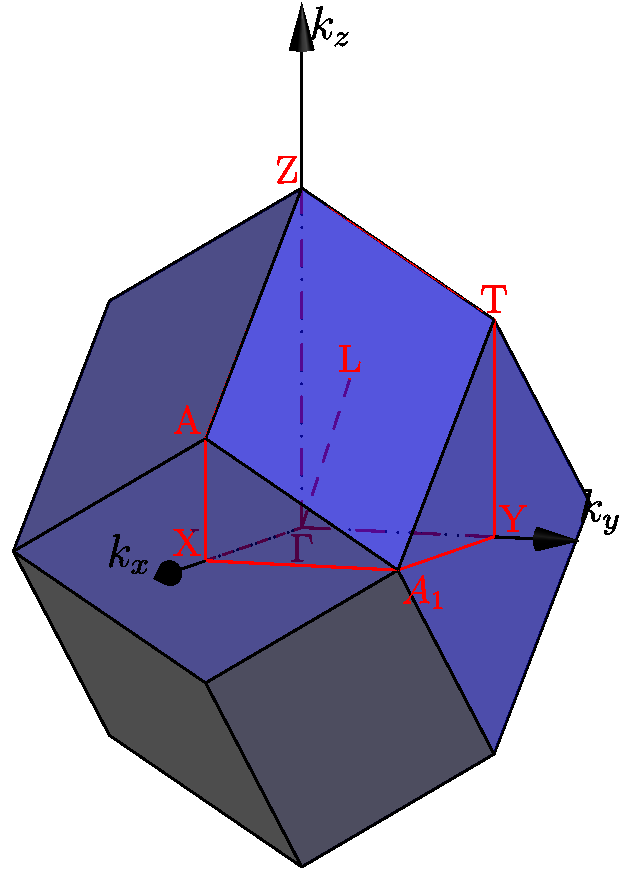
\includegraphics[width=5.5cm,angle=0]{images/ofc_17.png} \hspace{1cm}
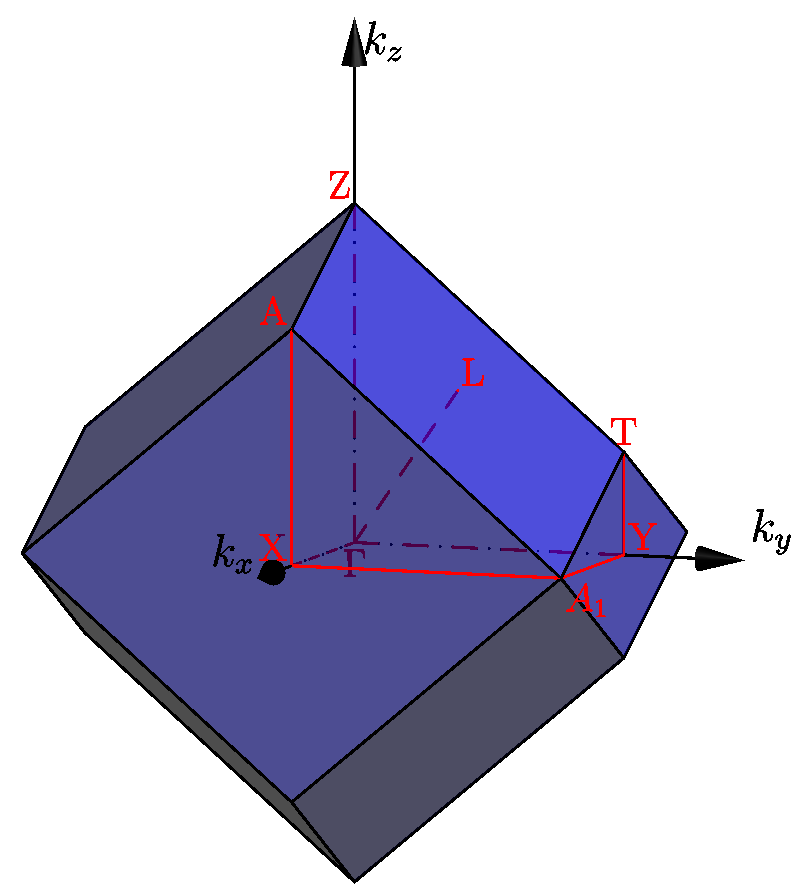
\includegraphics[width=7.5cm,angle=0]{images/ofc_18.png} 
\end{center}
The figures have been obtained with $b/a=1.333333333$ and $c/a=0.8$ 
(left part $a<b$) and with $b/a=0.66$ and $c/a=0.5508422$ (right part
$a>b$).

Finally the third possibility is that 
${1\over c^2} >{1\over a^2} + {1\over b^2}$:
\begin{center}
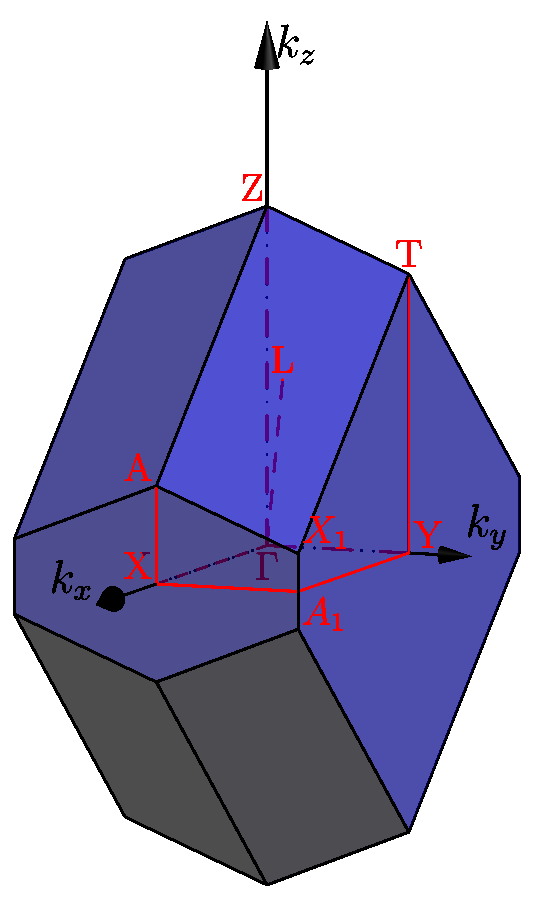
\includegraphics[width=5.0cm,angle=0]{images/ofc_11.png} \hspace{1cm}
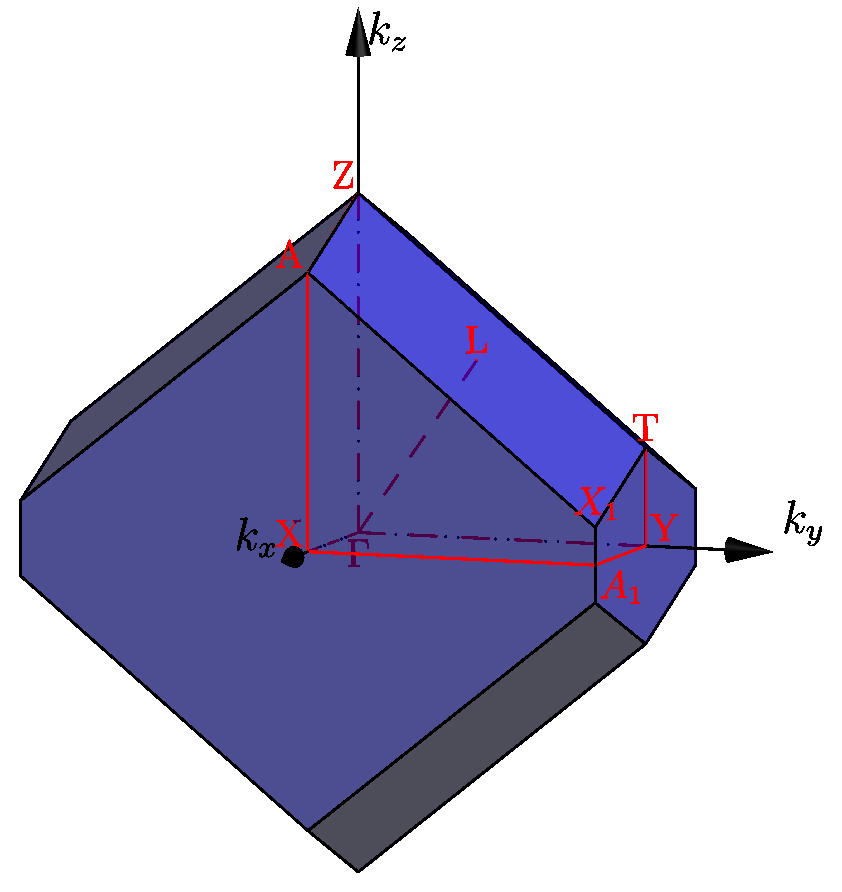
\includegraphics[width=7.5cm,angle=0]{images/ofc_12.png} 
\end{center}
The figures have been obtained with $b/a=2.0$ and $c/a=0.8$ (left part $a<b$),
and $b/a=0.5$ and $c/a=0.4$ (right part $a>b$).

\subsection{\texttt{ibrav=11}, body centered orthorhombic lattice}
The direct lattice vectors are:
\begin{eqnarray}
{\bf a}_1 &=& {a \over 2} (1, {b \over a}, {c \over a}), \nonumber \\
{\bf a}_2 &=& {a \over 2} (-1, {b \over a}, {c \over a}), \nonumber \\
{\bf a}_3 &=& {a \over 2} (-1, -{b \over a}, {c \over a}). \nonumber
\nonumber
\end{eqnarray}
while the reciprocal lattice vectors are:
\begin{eqnarray}
{\bf b}_1 &=& {2\pi \over a} (1, 0, {a \over c}), \nonumber \\
{\bf b}_2 &=& {2\pi \over a} (-1, {a \over b}, 0), \nonumber \\
{\bf b}_3 &=& {2\pi \over a} (0, -{a \over b}, {a \over c}). \nonumber
\nonumber
\end{eqnarray}
In this case the BZ has one shape that can be rotated in
different ways depending on the relative sizes of $a$, $b$, and $c$.
Similar orientations and BZ that differ only for the relative sizes of
the faces are obtained for the cases that have in common the longest side.
Therefore we distinguish the cases in which $a$ is the longest side 
and $b<c$ or $b>c$, the cases in which $b$ is the longest side and
$a<c$ or $a>c$ and the cases in which $c$ is the longest side and $a<b$
or $a>b$. We have $6$ distinct cases.

First we take $a$ as the longest side and show
on the left the case $b<c$ and on the right the case $b>c$:
\begin{center}
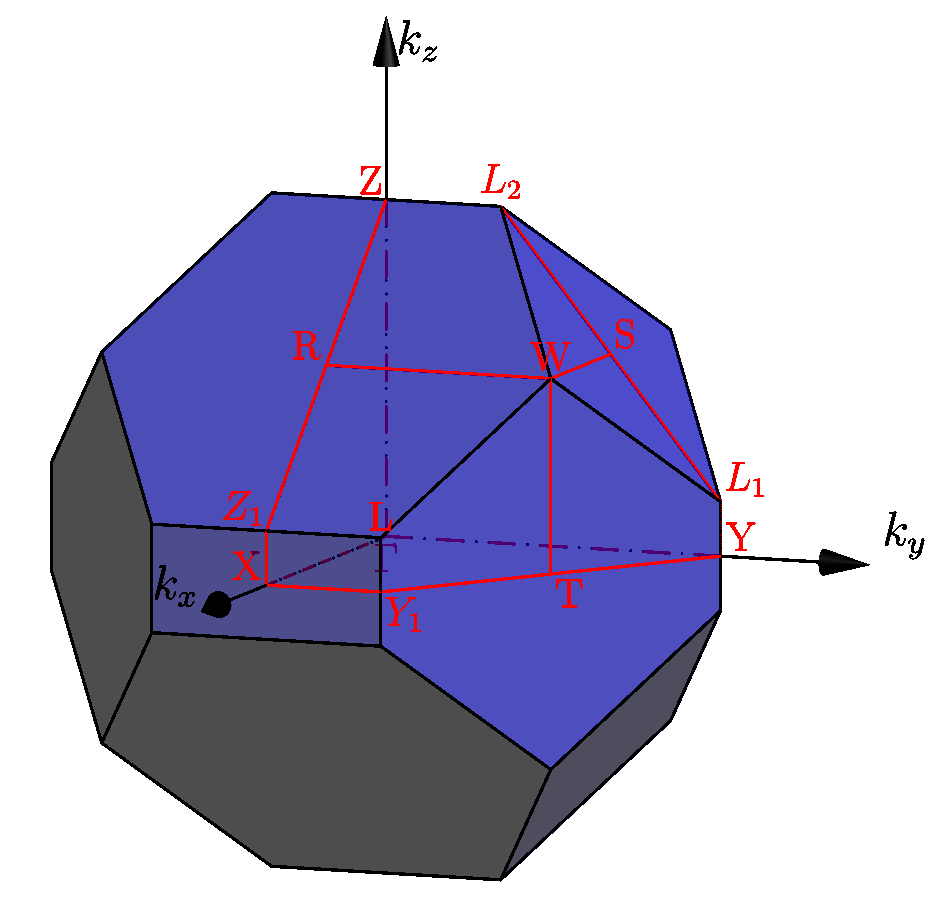
\includegraphics[width=7.5cm,angle=0]{images/bco_4.png} \hspace{1.0cm}
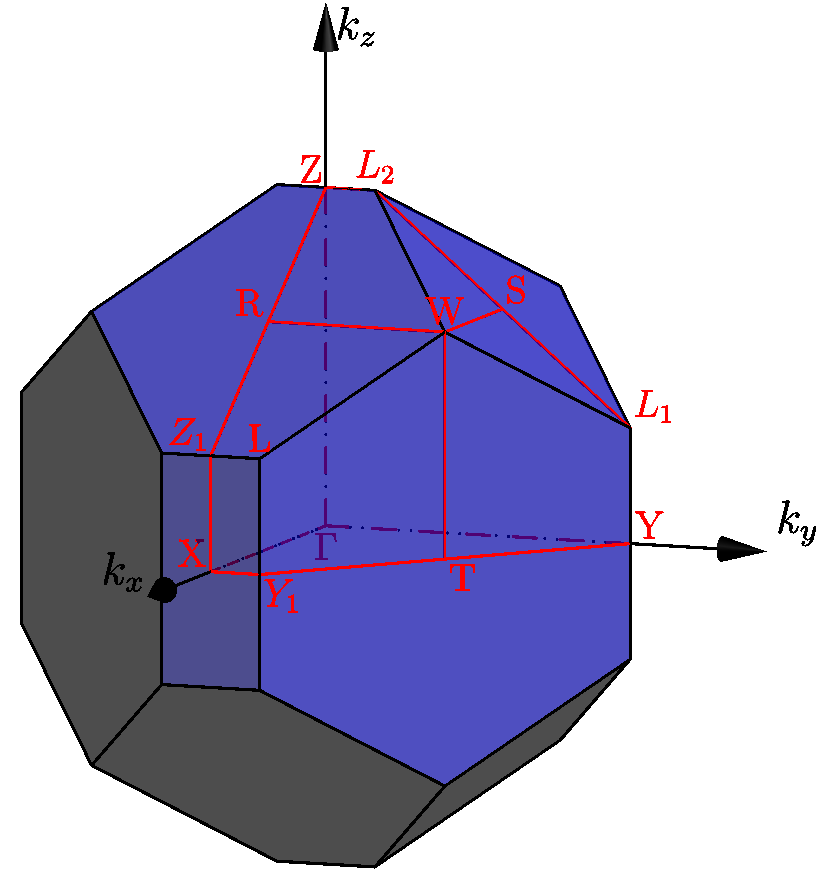
\includegraphics[width=7.5cm,angle=0]{images/bco_5.png}
\end{center}
The figures have been obtained with $b/a=0.7$ and $c/a=0.85$ (left part
$b<c$) and $b/a=0.85$ and $c/a=0.7$ (right part $b>c$).

Then we take $b$ as the longest side and show on the left the case 
in which $a<c$ and on the right the case in which $a>c$:
\begin{center}
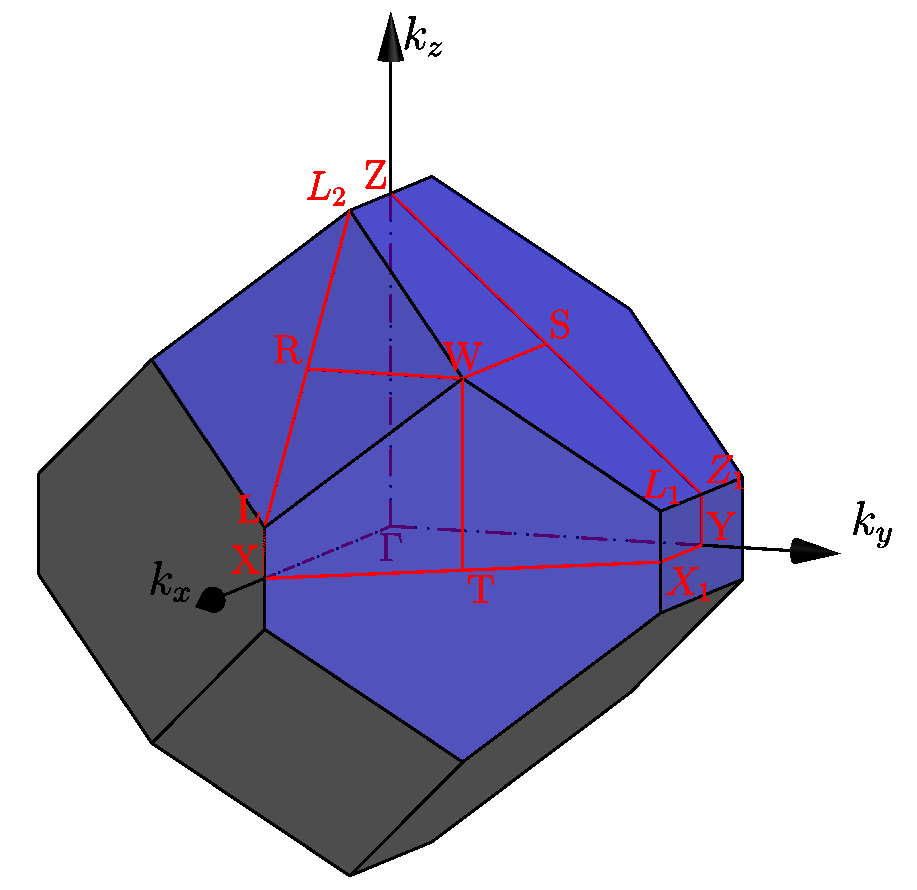
\includegraphics[width=7.5cm,angle=0]{images/bco_2.png}\hspace{1cm}
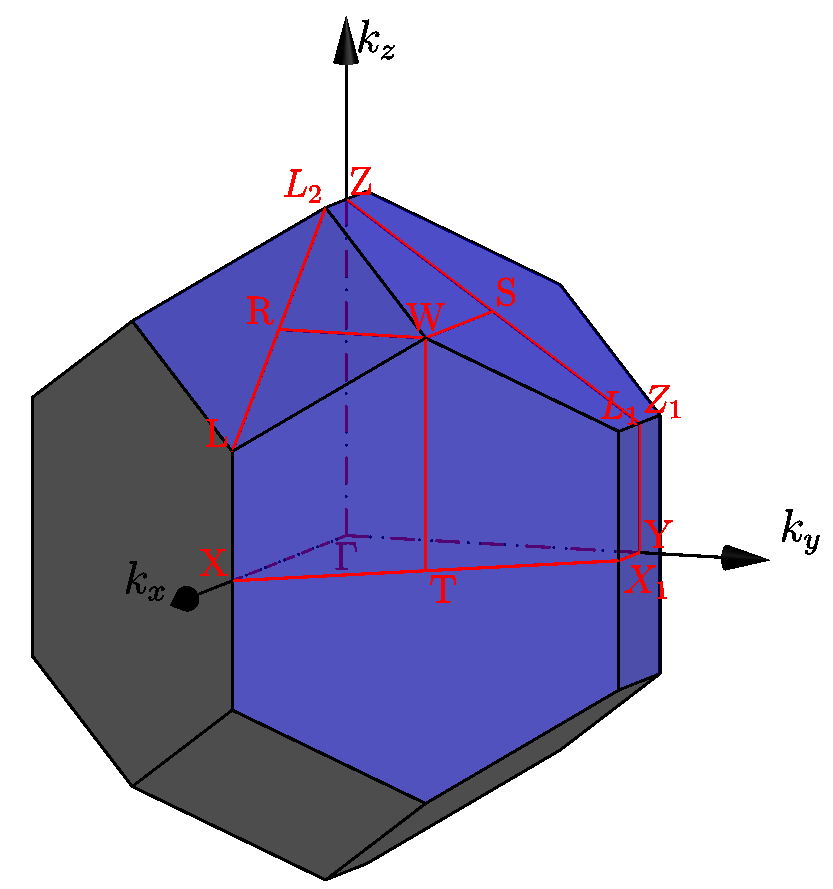
\includegraphics[width=7.cm,angle=0]{images/bco_3.png}
\end{center}
The figures have been obtained with $b/a=1.4$ and $c/a=1.2$ (left part $a<c$)
and $b/a=1.2$ and $c/a=0.8$ (right part $a>c$).

Finally we take $c$ as the longest side and show on the left the case in 
which $a<b$ and on the right the case in which $b<a$:
\begin{center}
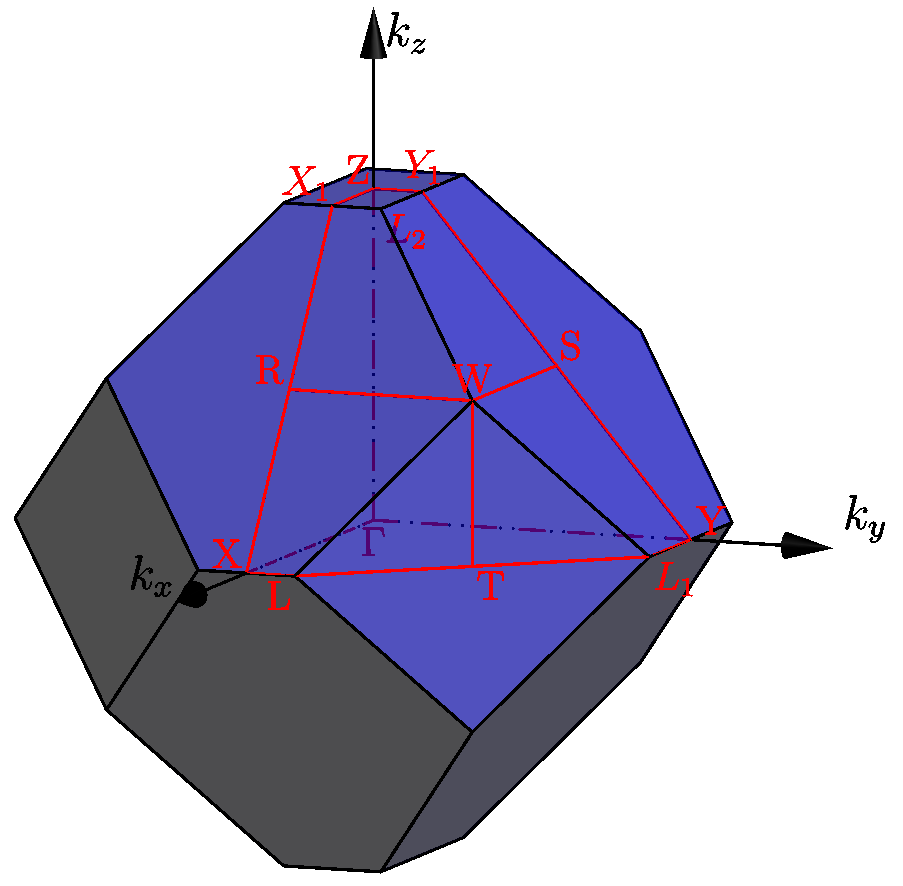
\includegraphics[width=7.5cm,angle=0]{images/bco_1.png} \hspace{1.0 cm}
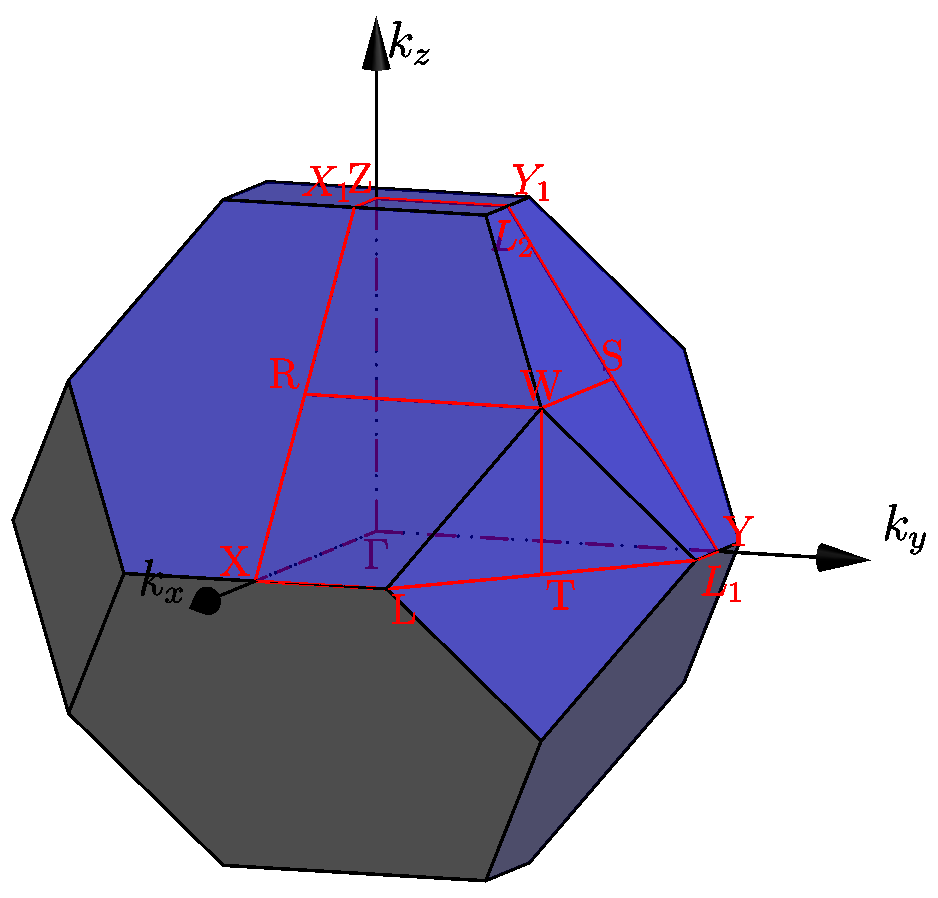
\includegraphics[width=7.5cm,angle=0]{images/bco_6.png}
\end{center}
The figures have been obtained with $b/a=1.2$ and $c/a=1.4$ (left part), and
$b/a=0.8$ and $c/a=1.2$ (right part).

\subsection{\texttt{ibrav=12}, simple monoclinic lattice, c unique}
The direct lattice vectors are:
\begin{eqnarray}
{\bf a}_1 &=& a (1, 0, 0), \nonumber \\
{\bf a}_2 &=& a ({b \over a} \cos{\gamma}, {b \over a}\sin{\gamma}, 0), \nonumber \\
{\bf a}_3 &=& a (0, 0, {c \over a}). 
\nonumber
\end{eqnarray}
while the reciprocal lattice vectors are:
\begin{eqnarray}
{\bf b}_1 &=& {2\pi \over a} (1, -{\cos{\gamma}\over \sin{\gamma}}, 0), \nonumber \\
{\bf b}_2 &=& {2\pi \over a} (0, {a \over b \sin{\gamma}}, 0), \nonumber \\
{\bf b}_3 &=& {2\pi \over a} (0, 0, {a \over c}). \nonumber
\end{eqnarray}
The Brillouin zone is: 
\begin{center}
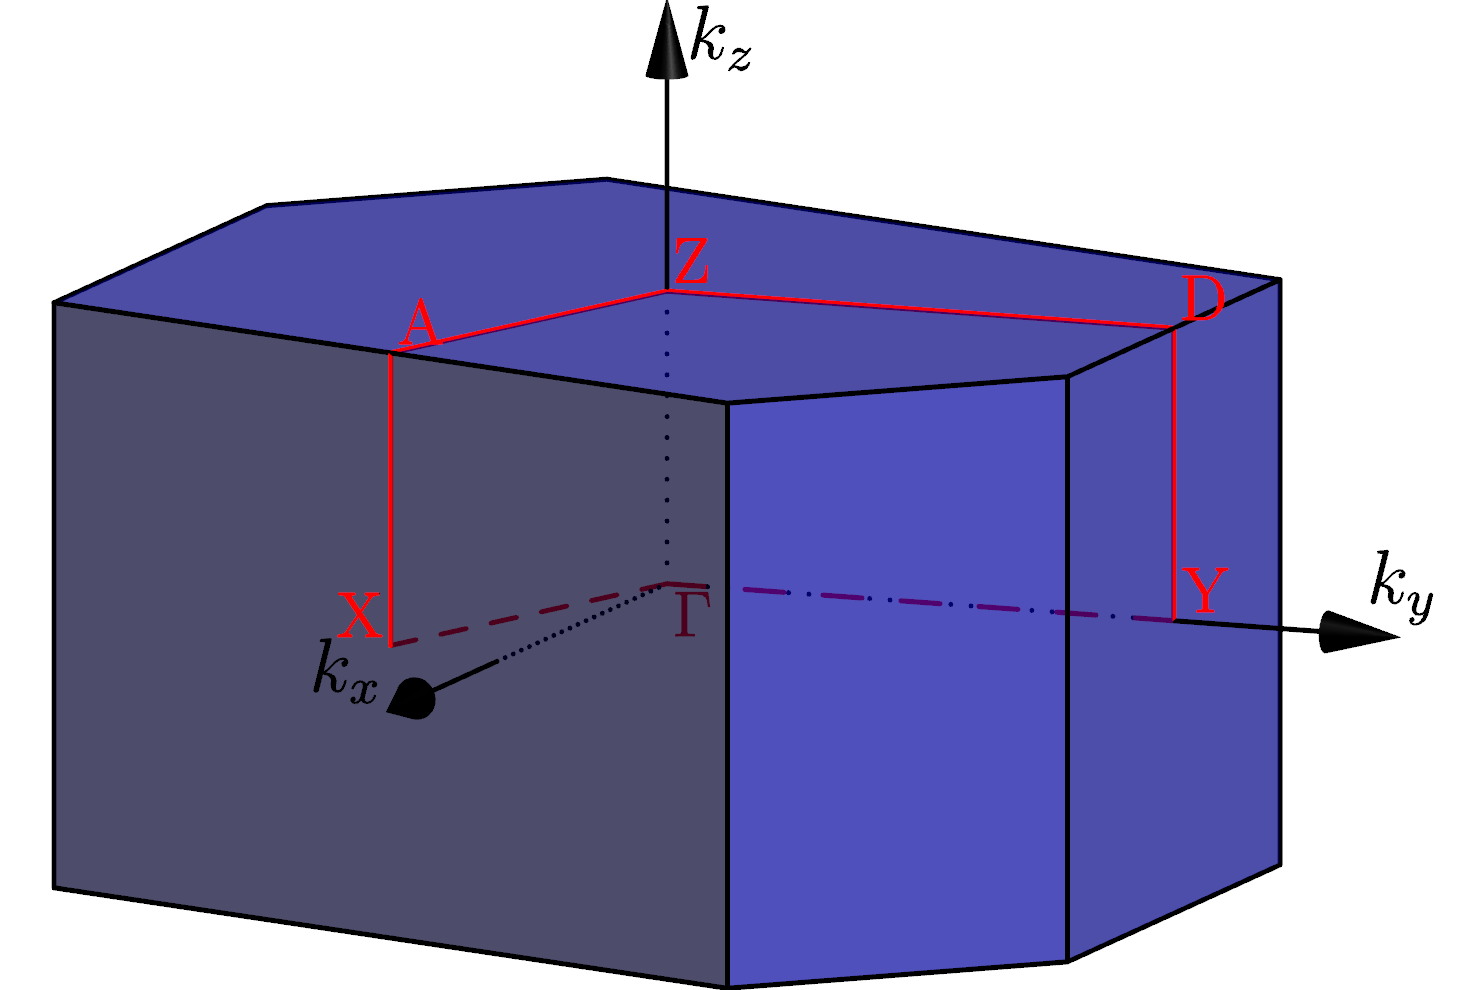
\includegraphics[width=7.5cm,angle=0]{images/monoc.png} 
\end{center}
The figure has been obtained with $b/a=0.8$, $c/a=1.4$ and $\cos{\gamma}=0.3$.

\subsection{\texttt{ibrav=-12}, simple monoclinic lattice, b unique}
The direct lattice vectors are:
\begin{eqnarray}
{\bf a}_1 &=& a (1, 0, 0), \nonumber \\
{\bf a}_2 &=& a (0, {b \over a}, 0), \nonumber \\
{\bf a}_3 &=& a ({c \over a} \cos{\beta}, 0, {c \over a}\sin{\beta}), \nonumber 
\end{eqnarray}
while the reciprocal lattice vectors are:
\begin{eqnarray}
{\bf b}_1 &=& {2\pi \over a} (1, 0, -{\cos{\beta}\over \sin{\beta}}), \nonumber \\
{\bf b}_2 &=& {2\pi \over a} (0, {a \over b}, 0), \nonumber \\
{\bf b}_3 &=& {2\pi \over a} (0, 0, {a \over c \sin{\beta}}). \nonumber
\end{eqnarray}
The Brillouin zone is: 
\begin{center}
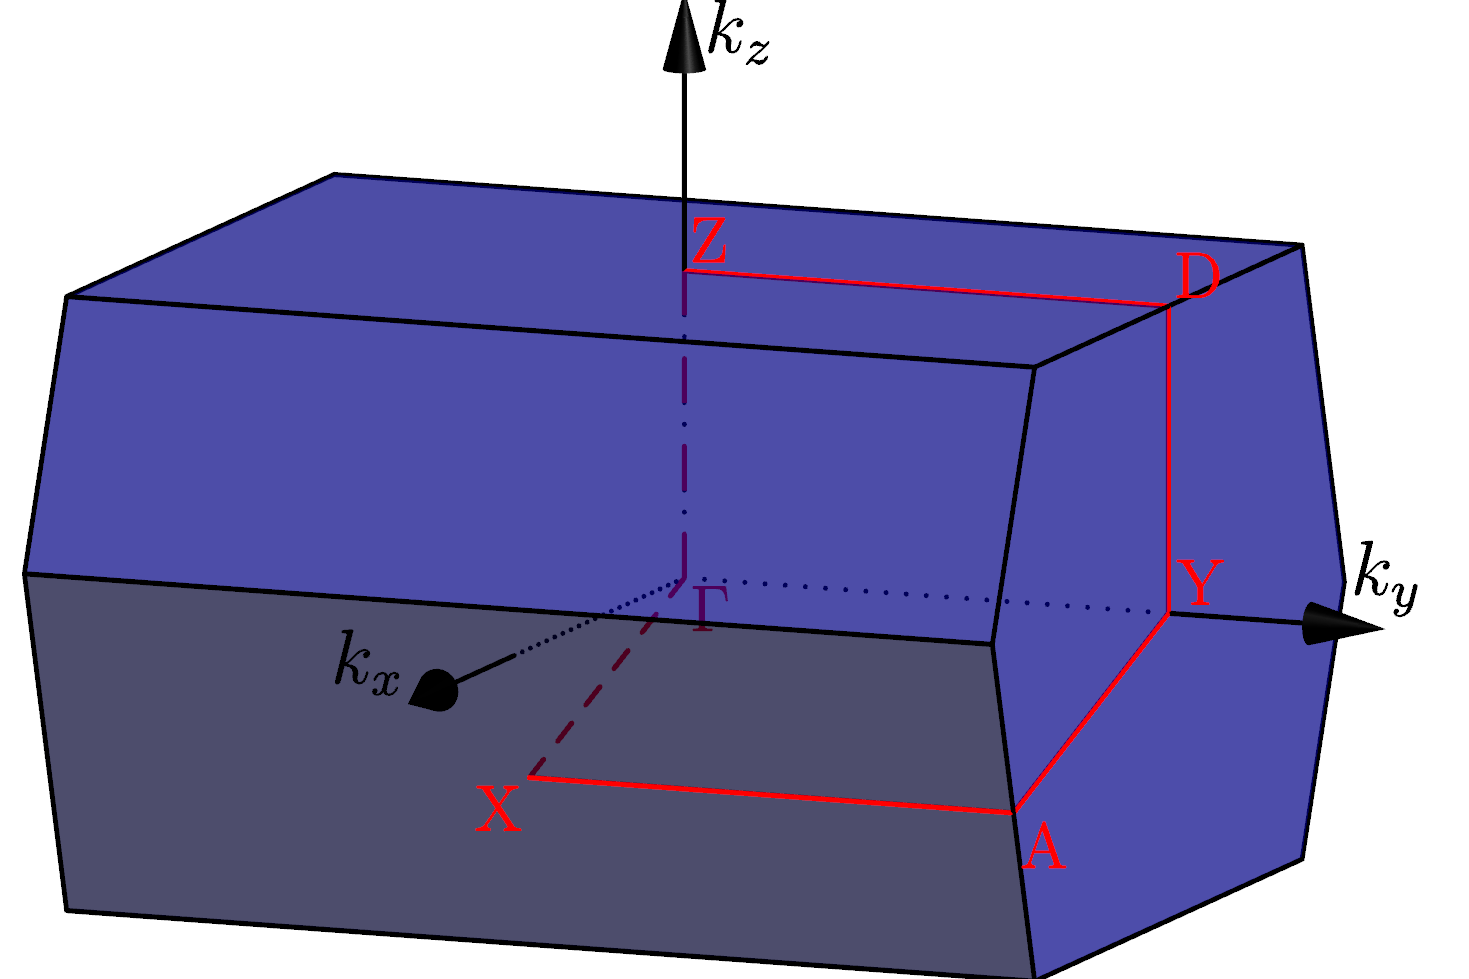
\includegraphics[width=7.5cm,angle=0]{images/monob.png} 
\end{center}
The figure has been obtained with $b/a=0.8$, $c/a=1.4$ and $\cos{\beta}=0.3$.


\subsection{\texttt{ibrav=13,14}, one-base centered monoclinic,
triclinic}
These lattices are not supported by this feature, you have to give
explicitly the coordinates of the path.

\section{Bibliography}

\noindent [1] G.F. Koster, Space groups and their representations, Academic press,
New York and London, (1957). 

\noindent [2] C.J. Bradley and A.P. Cracknell, The mathematical theory of symmetry
in solids, Oxford University Press, (1972).

\noindent [3] W. Setyawan and S. Curtarolo, Comp. Mat. Sci.  {\bf 49}, 299 (2010).

\noindent [4] E.S. Tasci, G. de la Flor, D. Orobengoa, C. Capillas, 
J.M. Perez-Mato, M.I. Aroyo, ``An introduction to the tools hosted in the 
Bilbao Crystallographic Server''. EPJ Web of Conferences 22 00009 (2012).

\end{document}
